\documentclass{article}
\usepackage[submission]{colm2026_conference}

\usepackage{microtype}
\usepackage{hyperref}
\usepackage{url}
\usepackage{booktabs}
\usepackage{graphicx}
\usepackage{amsmath,amsfonts}
\usepackage{multirow}
\usepackage{xcolor}
\usepackage{float}
\usepackage{lineno}

\definecolor{darkblue}{rgb}{0, 0, 0.5}
\hypersetup{colorlinks=true, citecolor=darkblue, linkcolor=darkblue, urlcolor=darkblue}

\DeclareMathOperator*{\argmax}{arg\,max}
\DeclareMathOperator*{\argmin}{arg\,min}

\title{When Should Multi-Agent LLM Systems Stop? \\ Topology-Aware Termination Dynamics}

\author{Anonymous Authors\\
Anonymous Institution\\
\texttt{anonymous@example.com}}

\newcommand{\fix}{\marginpar{FIX}}
\newcommand{\new}{\marginpar{NEW}}

\begin{document}

\ifcolmsubmission
\linenumbers
\fi

\maketitle

\begin{abstract}
When should multi-agent LLM systems stop working? As multi-agent coordination becomes a primary mechanism for scaling inference-time compute \citep{snell2024scaling,du2024debate}, a critical gap persists: stopping criteria remain topology-agnostic, applying the same fixed turn limits regardless of how agents coordinate, wasting computation on configurations that actively degrade output quality. Through 2,200+ controlled runs across 14 coordination patterns, we establish three results that overturn common assumptions. First, \emph{more agents can cost less}: decentralized routing beats larger sequential chains because topology---not system size---determines cost. Second, \emph{more computation can harm}: multi-agent debate quality degrades after the first round, while our hybrid marginal-utility criterion recovers up to 78\% of wasted tokens with zero quality loss. Third, \emph{difficulty trumps topology} by $7.8\times$: solo agents outperform multi-agent systems on easy tasks across most models, while coordination benefits only capable models on harder tasks. Validated across multiple models and providers---the largest cross-topology termination study to date---these results reveal that the field has been optimizing the wrong variable: task difficulty, not topology, determines when multi-agent coordination helps versus hurts. We release design guidelines and our experimental framework.
\end{abstract}

%=========================================================================
\section{Introduction}
\label{sec:intro}
%=========================================================================

\subsection{Why Termination Matters}

Multi-agent LLM systems---AutoGen \citep{wu2023autogen}, CrewAI, LangGraph---coordinate specialized agents through topologies from round-robin chains to debate protocols. As these systems scale, a critical cost problem emerges: multi-agent coordination incurs 3--17$\times$ token overhead compared to single-agent baselines, and poorly calibrated stopping wastes up to 78\% of computation on configurations that actively degrade output quality. Yet the fundamental question of \emph{when these systems should stop} remains unexplored.

This connects to \emph{inference-time compute scaling} \citep{snell2024scaling}: multi-agent coordination is structured test-time compute allocation, and the optimal stopping point defines the saturation boundary beyond which additional computation yields diminishing returns. Current practice relies on rudimentary criteria applied uniformly---fixed turn limits, keyword detection, and timeouts---ignoring that \emph{the optimal stopping point depends on how agents coordinate}. A round-robin may finish in two turns, while a debate may need several rounds. We term this mismatch \emph{termination regret}: the gap between actual and optimal stopping.

\subsection{Our Approach}
\vspace{-1mm}

To systematically investigate this problem, we conduct the largest cross-topology termination study to date: 2,200+ controlled runs across 14 coordination patterns in six topology categories, spanning seven experiments that progress from efficiency measurement through quality tracking, convergence detection, error attribution, adaptive stopping, cost prediction, and difficulty interaction. We validate across multiple models from multiple providers, including open-weight models, to ensure generalizability.

\subsection{Research Questions}
\vspace{-1mm}

Our experiments address seven questions:
\textbf{RQ1}: How do termination dynamics differ across topologies?
\textbf{RQ2}: Can per-turn quality trajectories detect termination regret?
\textbf{RQ3}: Do feedback patterns exhibit convergence signals?
\textbf{RQ4}: Do topologies produce characteristic error patterns?
\textbf{RQ5}: Does marginal utility $\Delta U(t)$ converge as a stopping signal?
\textbf{RQ6}: Can topology features predict runtime costs?
\textbf{RQ7}: How does task difficulty moderate topology choice?

\subsection{Contributions}
\vspace{-1mm}

Our study yields seven contributions:
\textbf{(1)}~The first cross-topology termination study across 14 patterns in six categories; prior work covers $\leq$3 \citep{cemri2025why,hu2025when}.
\textbf{(2)}~A \emph{termination regret} metric via per-turn G-Eval \citep{liu2023geval} quality trajectories, revealing that regret varies 13$\times$ across topologies.
\textbf{(3)}~Claim-level convergence detection extending \citet{hu2025when}'s debate-only approach to all topologies via sentence-transformer embeddings \citep{reimers2019sentence}.
\textbf{(4)}~A pattern-specific error taxonomy linking topology to failure mode.
\textbf{(5)}~A hybrid keyword+marginal-utility stopping criterion ($\Delta U(t) = \Delta Q(t) - \lambda \Delta C(t) \to 0$) that recovers 78\% of wasted tokens for unreliable topologies with zero quality loss.
\textbf{(6)}~Cost prediction from topology features ($R^2$=0.54).
\textbf{(7)}~A difficulty--capability interaction showing that task difficulty explains $7.8\times$ more variance than topology choice ($\eta^2_H$=0.364 vs.\ 0.046), reframing the design question from \emph{which topology} to \emph{whether multi-agent coordination is warranted}.

%=========================================================================
\vspace{-1mm}
\section{Background and Related Work}
\label{sec:background}
\vspace{-1mm}
%=========================================================================

\subsection{Multi-Agent Coordination Topologies}
\vspace{-1mm}

Grounded in MAS topology theory \citep{masterman2025landscape}, we organize 13 coordination patterns into six categories including a single-agent baseline (Figure~\ref{fig:taxonomy}):
\textbf{(A)~Chain}---fixed round-robin cycles (RR-2/3/4);
\textbf{(B1)~Centralized Star}---coordinator routes to specialists (Sel-3/4);
\textbf{(B2)~Decentralized Mesh}---agents self-route via tool calls (Swm-3/4);
\textbf{(C)~Structured Feedback}---reflection or debate loops (Refl-2/3, Deb-3/4);
\textbf{(D)~Composed}---pipeline or mixture-of-agents (Pipe, MoA).

Prior frameworks implement subsets: AutoGen \citep{wu2023autogen} (round-robin, selector, swarm), DyTopo \citep{lu2026dytopo} (dynamic switching), MoA \citep{li2025moa} (layered aggregation). G-Designer \citep{zhang2025gdesigner} generates task-specific topologies via graph auto-encoders. \citet{xiong2025scaling} evaluate 5 architectures across 180 configurations. AgentDropout \citep{wang2025agentdropout} optimizes communication graphs; AgentsNet \citep{grotschla2025agentsnet} studies graph-based coordination; MultiAgentBench \citep{zhu2025multiagentbench} evaluates collaboration dynamics. Our study focuses specifically on \emph{termination dynamics}---when to stop, not how to coordinate.

\subsection{Stopping Criteria in LLM Systems}
\vspace{-1mm}

\textbf{Single-agent.} REFRAIN \citep{sun2025refrain} addresses CoT ``overthinking'' via UCB-controlled stop discriminator ($-$20--55\% tokens). \textbf{Multi-agent.} \citet{du2024debate} establish multi-agent debate as an inference-time scaling mechanism; \citet{chen2024more} show majority voting across agents improves with count. For stopping: \citet{hu2025when} propose KS-test stability detection for debate; Aegean \citep{ruan2025reaching} uses quorum-based consensus ($-$1.2--20$\times$ latency); \citet{cemri2025why} identify termination as a failure category; SupervisorAgent \citep{lin2025stop} applies LLM-free context filtering ($-$29\% tokens). \textbf{Gap.} No prior work systematically compares termination dynamics across $>$3 coordination topologies. We bridge this gap with 14 patterns across six categories (Table~\ref{tab:related} in Appendix~\ref{app:related_table}).

We adopt G-Eval \citep{liu2023geval} as our per-turn quality metric (accuracy, completeness, coherence, usefulness, overall; 1--5 scale), using Claude Sonnet~4.5 as the judge model.

%=========================================================================
\vspace{-1mm}
\section{Methodology}
\label{sec:methodology}
\vspace{-1mm}
%=========================================================================

\subsection{Pattern Taxonomy}
\vspace{-1mm}

We study 13 coordination patterns plus a single-agent baseline (Category~S) organized into six categories (Figure~\ref{fig:taxonomy}), sharing \texttt{TERMINATE} keyword detection and \texttt{max\_messages}=25 as safety bound. Table~\ref{tab:patterns} details configurations.

\begin{figure}[t]
\centering
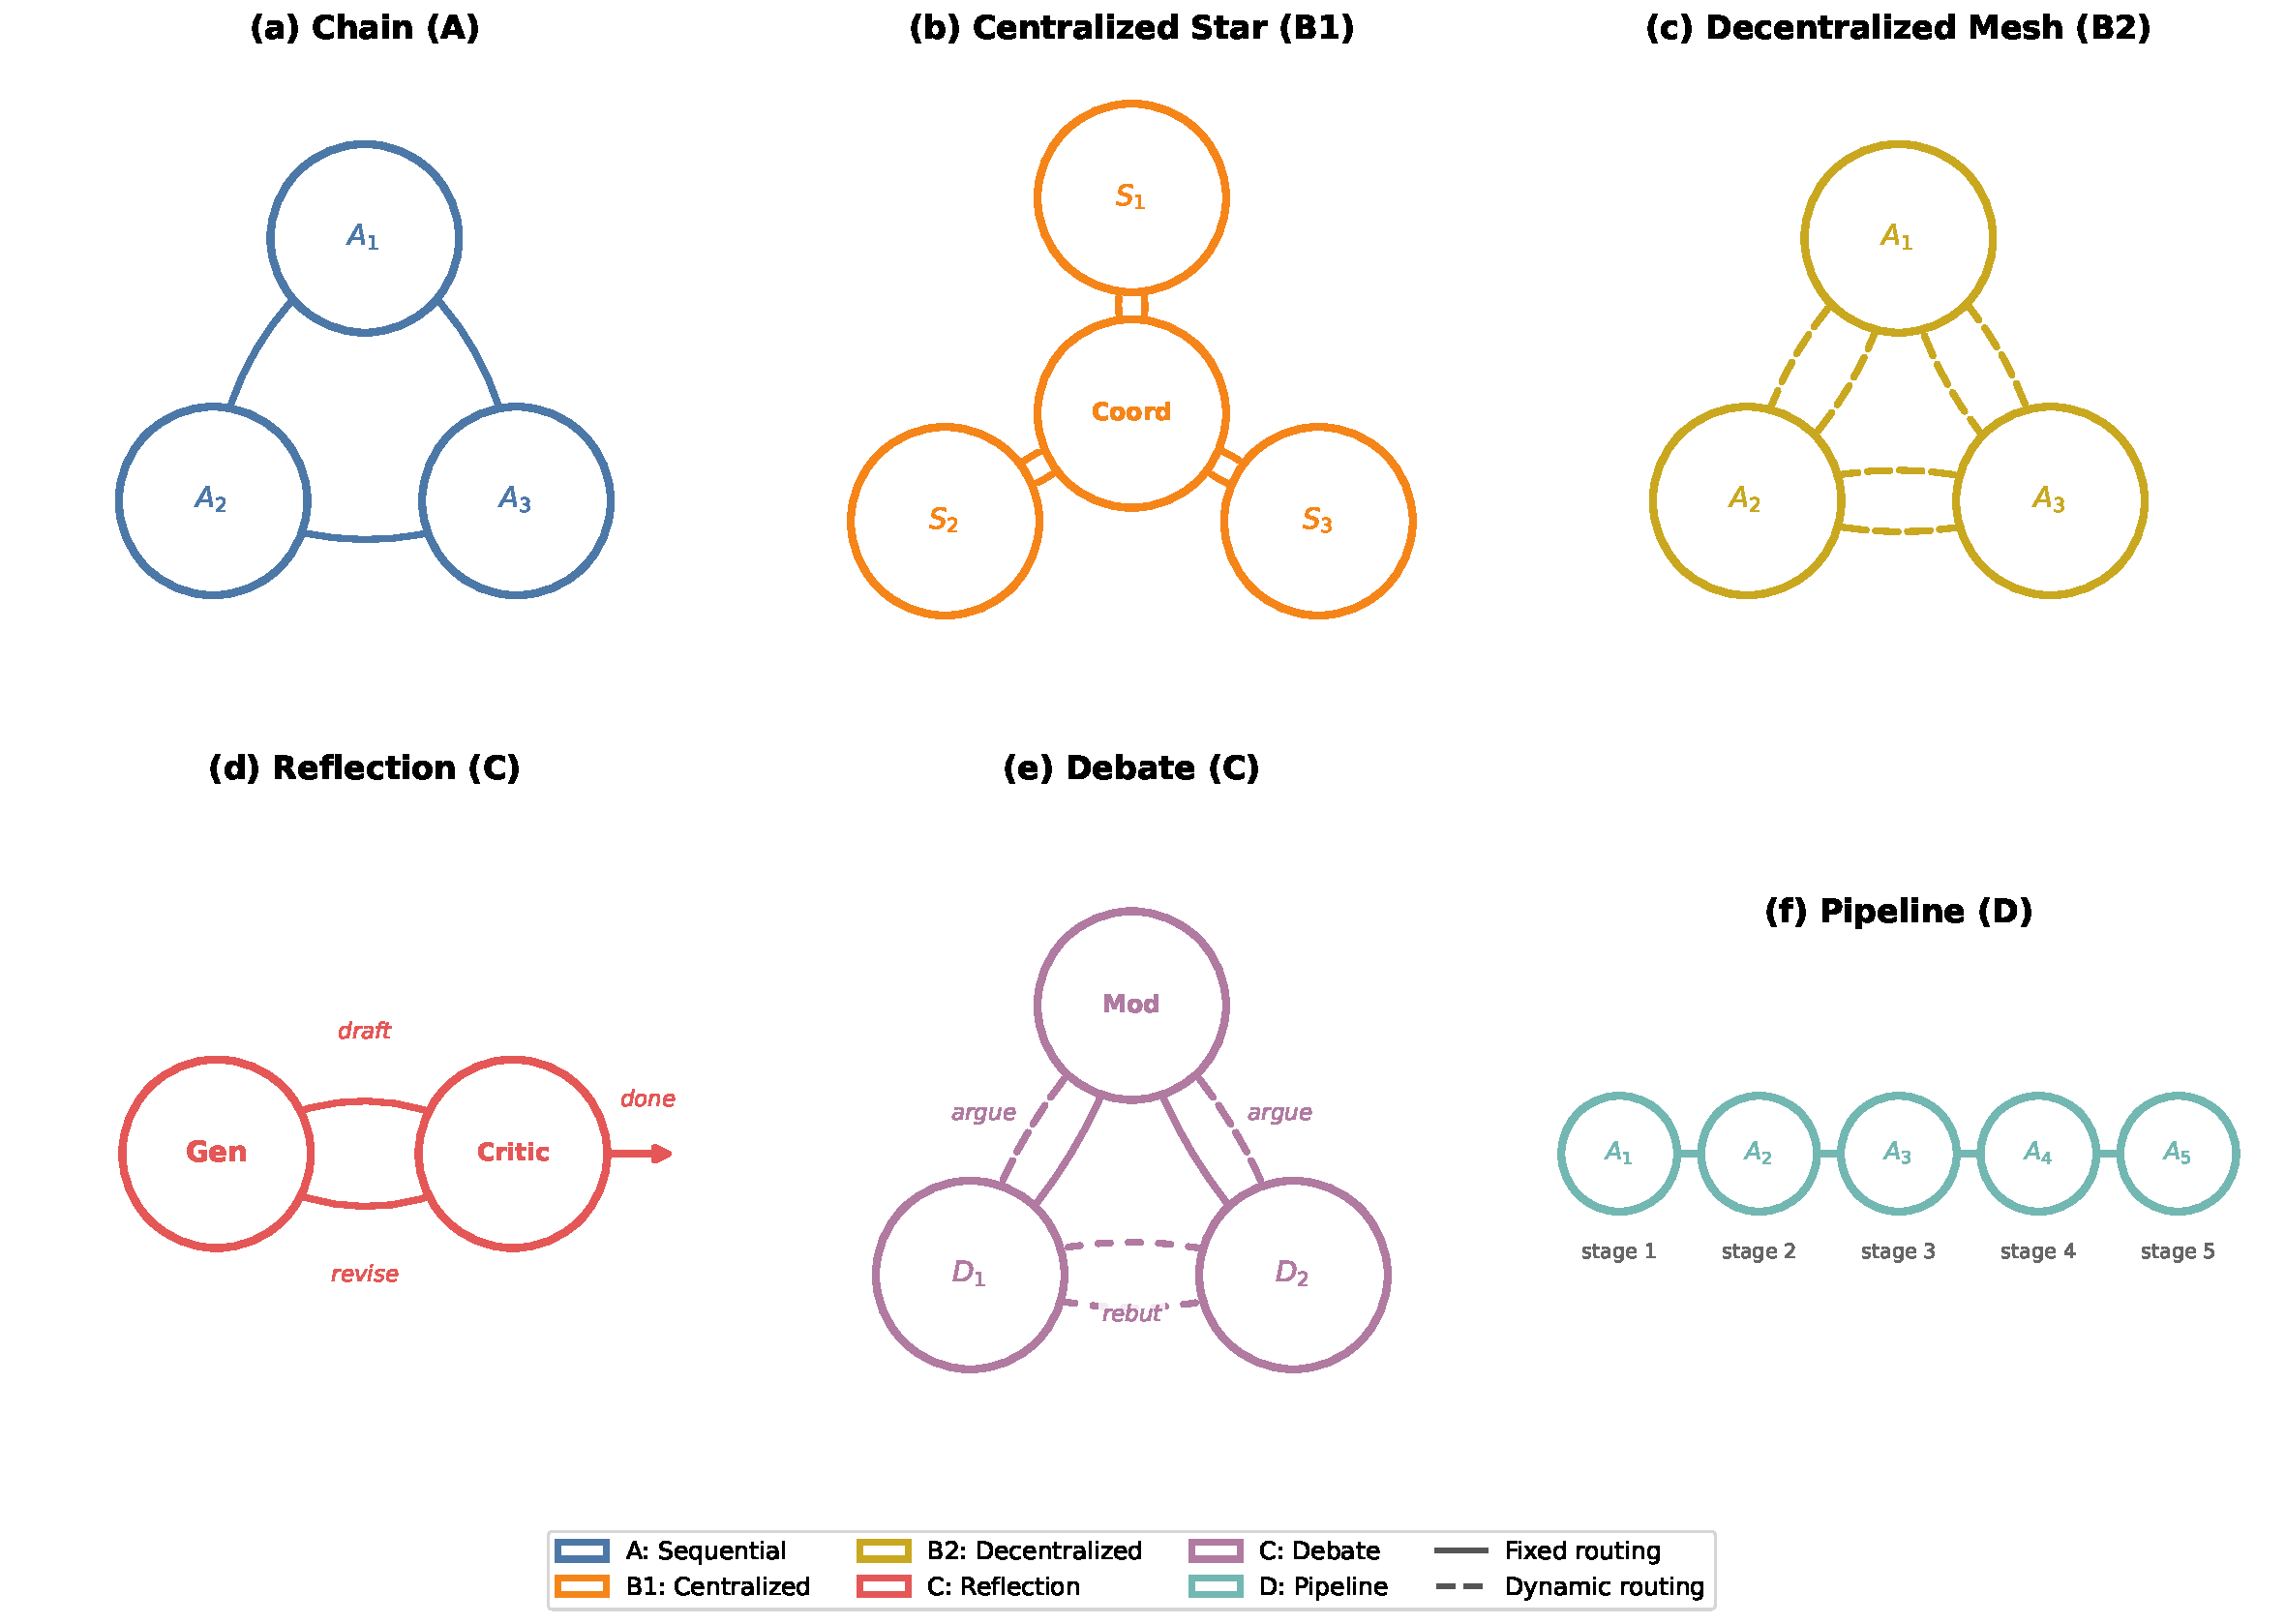
\includegraphics[width=\linewidth]{fig1_taxonomy.pdf}
\caption{Six representative coordination topologies. (a)~Chain: fixed round-robin cycle. (b)~Centralized star: coordinator dynamically routes to specialists. (c)~Decentralized mesh: agents self-route via tool calls. (d)~Reflection: generator-critic loop with approval exit. (e)~Debate: argumentation with moderator synthesis. (f)~Pipeline: staged sequential refinement. Solid lines = fixed routing; dashed = dynamic routing.}
\label{fig:taxonomy}
\end{figure}

\begin{table}[t]
\centering
\caption{Pattern configurations. Agent counts exclude the coordinator in B1/C debate patterns (shown as $n$+1).}
\label{tab:patterns}
{\small
\begin{tabular}{@{}llcll@{}}
\toprule
\textbf{Pattern} & \textbf{Cat.} & \textbf{Agents} & \textbf{Routing} & \textbf{Termination} \\
\midrule
Solo & S & 1 & None & Keyword \\
RR-2 & A & 2 & Fixed RR & Keyword/max \\
RR-3 & A & 3 & Fixed RR & Keyword/max \\
RR-4 & A & 4 & Fixed RR & Keyword/max \\
Sel-3 & B1 & 3+1 & LLM-routed & Keyword/max \\
Sel-4 & B1 & 4+1 & LLM-routed & Keyword/max \\
Swm-3 & B2 & 3 & Self-routing & Keyword/max \\
Swm-4 & B2 & 4 & Self-routing & Keyword/max \\
Refl-2 & C & 2 & Fixed+feedback & Keyword/max \\
Refl-3 & C & 3 & Fixed+feedback & Keyword/max \\
Deb-3 & C & 3+1 & Moderated & Keyword/max \\
Deb-4 & C & 4+1 & Moderated & Keyword/max \\
Pipe & D & 5 & Sequential stages & Per-stage \\
MoA & D & 4 & Fan-out/agg. & Aggregator \\
\bottomrule
\end{tabular}
}
\end{table}

\subsection{Task Suite}
\vspace{-1mm}

We design 25 tasks spanning 4 cognitive types (factual, analytical, creative, technical) across 9 domains (science, CS, history, philosophy, law/politics, gaming, engineering, business, medicine). This diversity is deliberate: domain-specific topology interactions (e.g., debate excels in politics but wastes tokens in factual domains) can only emerge from broad coverage. For Experiment~07, we further construct a 15-task difficulty-graded subset across 5 domains (science, CS, history, engineering, business), each with easy (factual recall), medium (comparative analysis), and hard (creative multi-constraint design) variants (Table~\ref{tab:difficulty_tasks} in Appendix~\ref{app:difficulty_tasks}). Full task descriptions in Appendix~\ref{app:tasks}.

\subsection{Experimental Framework}
\vspace{-1mm}

All experiments use AutoGen with Claude Haiku 4.5 as the base model. Cross-model generalizability is assessed via GPT-4o-mini replication (Section~\ref{sec:cross_model}) and six-model cross-validation from four providers. Metrics: duration, turns, tokens (prompt/completion), stop reason, quality (Exp02), convergence (Exp03). All reported significant effects survive Benjamini-Hochberg FDR correction \citep{benjamini1995controlling} at $q < 0.05$.

\subsection{Seven Experiments}
\vspace{-1mm}

\textbf{Exp01}: Pattern Efficiency---780 runs (13 patterns $\times$ 20 tasks $\times$ 3 repeats).
\textbf{Exp02}: Termination Quality---100 runs (5 patterns $\times$ 20 tasks, 276 turn-level G-Eval scores).
\textbf{Exp03}: Convergence Detection---Sentence-BERT on 200 runs (8 patterns).
\textbf{Exp04}: Error Attribution---structural classification from Exp01/02.
\textbf{Exp05}: Adaptive Termination---800 runs (8 patterns $\times$ 25 tasks $\times$ 4 conditions).
\textbf{Exp06}: Cost Prediction---regression on Exp01 data (5-fold CV + holdout).
\textbf{Exp07}: Difficulty Interaction---743 scored runs (5 patterns $\times$ 15 tasks $\times$ 6 models; 3 repeats for two models, 1 for four).

%=========================================================================
\vspace{-1mm}
\section{Results}
\label{sec:results}
\vspace{-1mm}
%=========================================================================

\subsection{Experiment 01: Pattern Efficiency (RQ1)}
\label{sec:exp01}

We executed 780 runs (13 patterns $\times$ 20 tasks $\times$ 3 repeats). The solo baseline (1,287 tokens, 18.7s) establishes a 3.3--6.1$\times$ coordination overhead across all multi-agent categories (Appendix Table~\ref{tab:solo_baseline}).

\paragraph{Finding 1: Multi-agent coordination incurs 3.3--6.1$\times$ overhead.} Even swm3 (3.26$\times$) consumes $>$3$\times$ solo tokens, anchoring all subsequent comparisons. Table~\ref{tab:cross_category} ranks 12 patterns by cost (rr4 excluded: 71.7\% error rate; Section~\ref{sec:exp04}).

\begin{table}[t]
\centering
\caption{Cross-category efficiency (12 multi-agent patterns + solo; rr4 excluded: 71.7\% error rate). SDs in Appendix~\ref{app:stats}.}
\label{tab:cross_category}
{\small
\begin{tabular}{@{}llcrrrrr@{}}
\toprule
\textbf{Pattern} & \textbf{Cat.} & \textbf{Agents} & \textbf{Dur.(s)} & \textbf{Tokens} & \textbf{Out/Turn} & \textbf{vs.\ solo} \\
\midrule
solo & S & 1 & 18.7 & 1,287 & -- & 1.00$\times$ \\
swm3 & B2 & 3 & 75.2 & 4,196 & 337 & 3.26$\times$ \\
rr2 & A & 2 & 52.4 & 4,759 & 1,583 & 3.70$\times$ \\
refl2 & C & 2 & 60.2 & 5,237 & 1,732 & 4.07$\times$ \\
sel3 & B1 & 3+1 & 115.2 & 7,851 & 2,114 & 6.10$\times$ \\
deb3 & C & 3+1 & 156.6 & 9,313 & 1,691 & 7.23$\times$ \\
rr3 & A & 3 & 96.6 & 10,121 & 1,701 & 7.86$\times$ \\
sel4 & B1 & 4+1 & 161.9 & 11,595 & 2,616 & 9.01$\times$ \\
deb4 & C & 4+1 & 180.9 & 11,637 & 1,448 & 9.04$\times$ \\
refl3 & C & 3 & 120.2 & 12,095 & 2,537 & 9.40$\times$ \\
swm4 & B2 & 4 & 185.0 & 13,321 & 330 & 10.35$\times$ \\
pipe & D & 5 & 129.6 & 13,856 & 2,325 & 10.76$\times$ \\
moa & D & 4 & 103.0 & 22,333 & 2,494 & 17.35$\times$ \\
\bottomrule
\end{tabular}
}
\vspace{-1mm}
\end{table}

\paragraph{Category A (Sequential).} Adding agents doubles duration (rr3/rr2=1.84$\times$) and tokens (2.13$\times$), driven by superlinear input growth (2.59$\times$). Errors scale superlinearly: rr2=8.3\% $\to$ rr3=23.3\% $\to$ rr4=71.7\%.

\paragraph{Category B (Dynamic Routing).} Selector and swarm exhibit opposite scaling: selector is \textbf{sub-linear} (sel4/sel3=1.48$\times$) with few long turns (2,114--2,616 out tok/turn), while swarm is \textbf{super-linear} (swm4/swm3=3.17$\times$) with many short handoffs (330--337 tok/turn). At $n$=3, swm3 is 47\% cheaper than sel3; at $n$=4, swm4 is 15\% costlier than sel4---implying swarm for small systems, selector for larger ones.

\paragraph{Finding 2: swm3 achieves best token efficiency.} swm3 (3 agents, 4,196 tokens) is 12\% cheaper than rr2 (2 agents, 4,759 tokens)---more agents can cost less when routing avoids full-context broadcasting.

\paragraph{Categories C--D.} Reflection scales super-linearly (refl3/refl2=2.31$\times$); debate sub-linearly (deb4/deb3=1.25$\times$). MoA is costliest (22,333 tokens) but 21\% faster than pipe via parallelism. Kruskal-Wallis ($N$=718): $p<0.001$ for all metrics; cost hierarchy $\text{A} \approx \text{B2} < \text{B1} \approx \text{C} \ll \text{D}$ (Appendix Table~\ref{tab:pairwise}).

\paragraph{Implication.} These scaling differences mean practitioners face a fundamental design trade-off: decentralized routing (swarm) is cheapest at small scale but scales poorly, while centralized routing (selector) has higher fixed cost but scales gracefully. The practical consequence is that \emph{system size should inform topology choice, not the reverse}.

\begin{figure}[t]
\centering
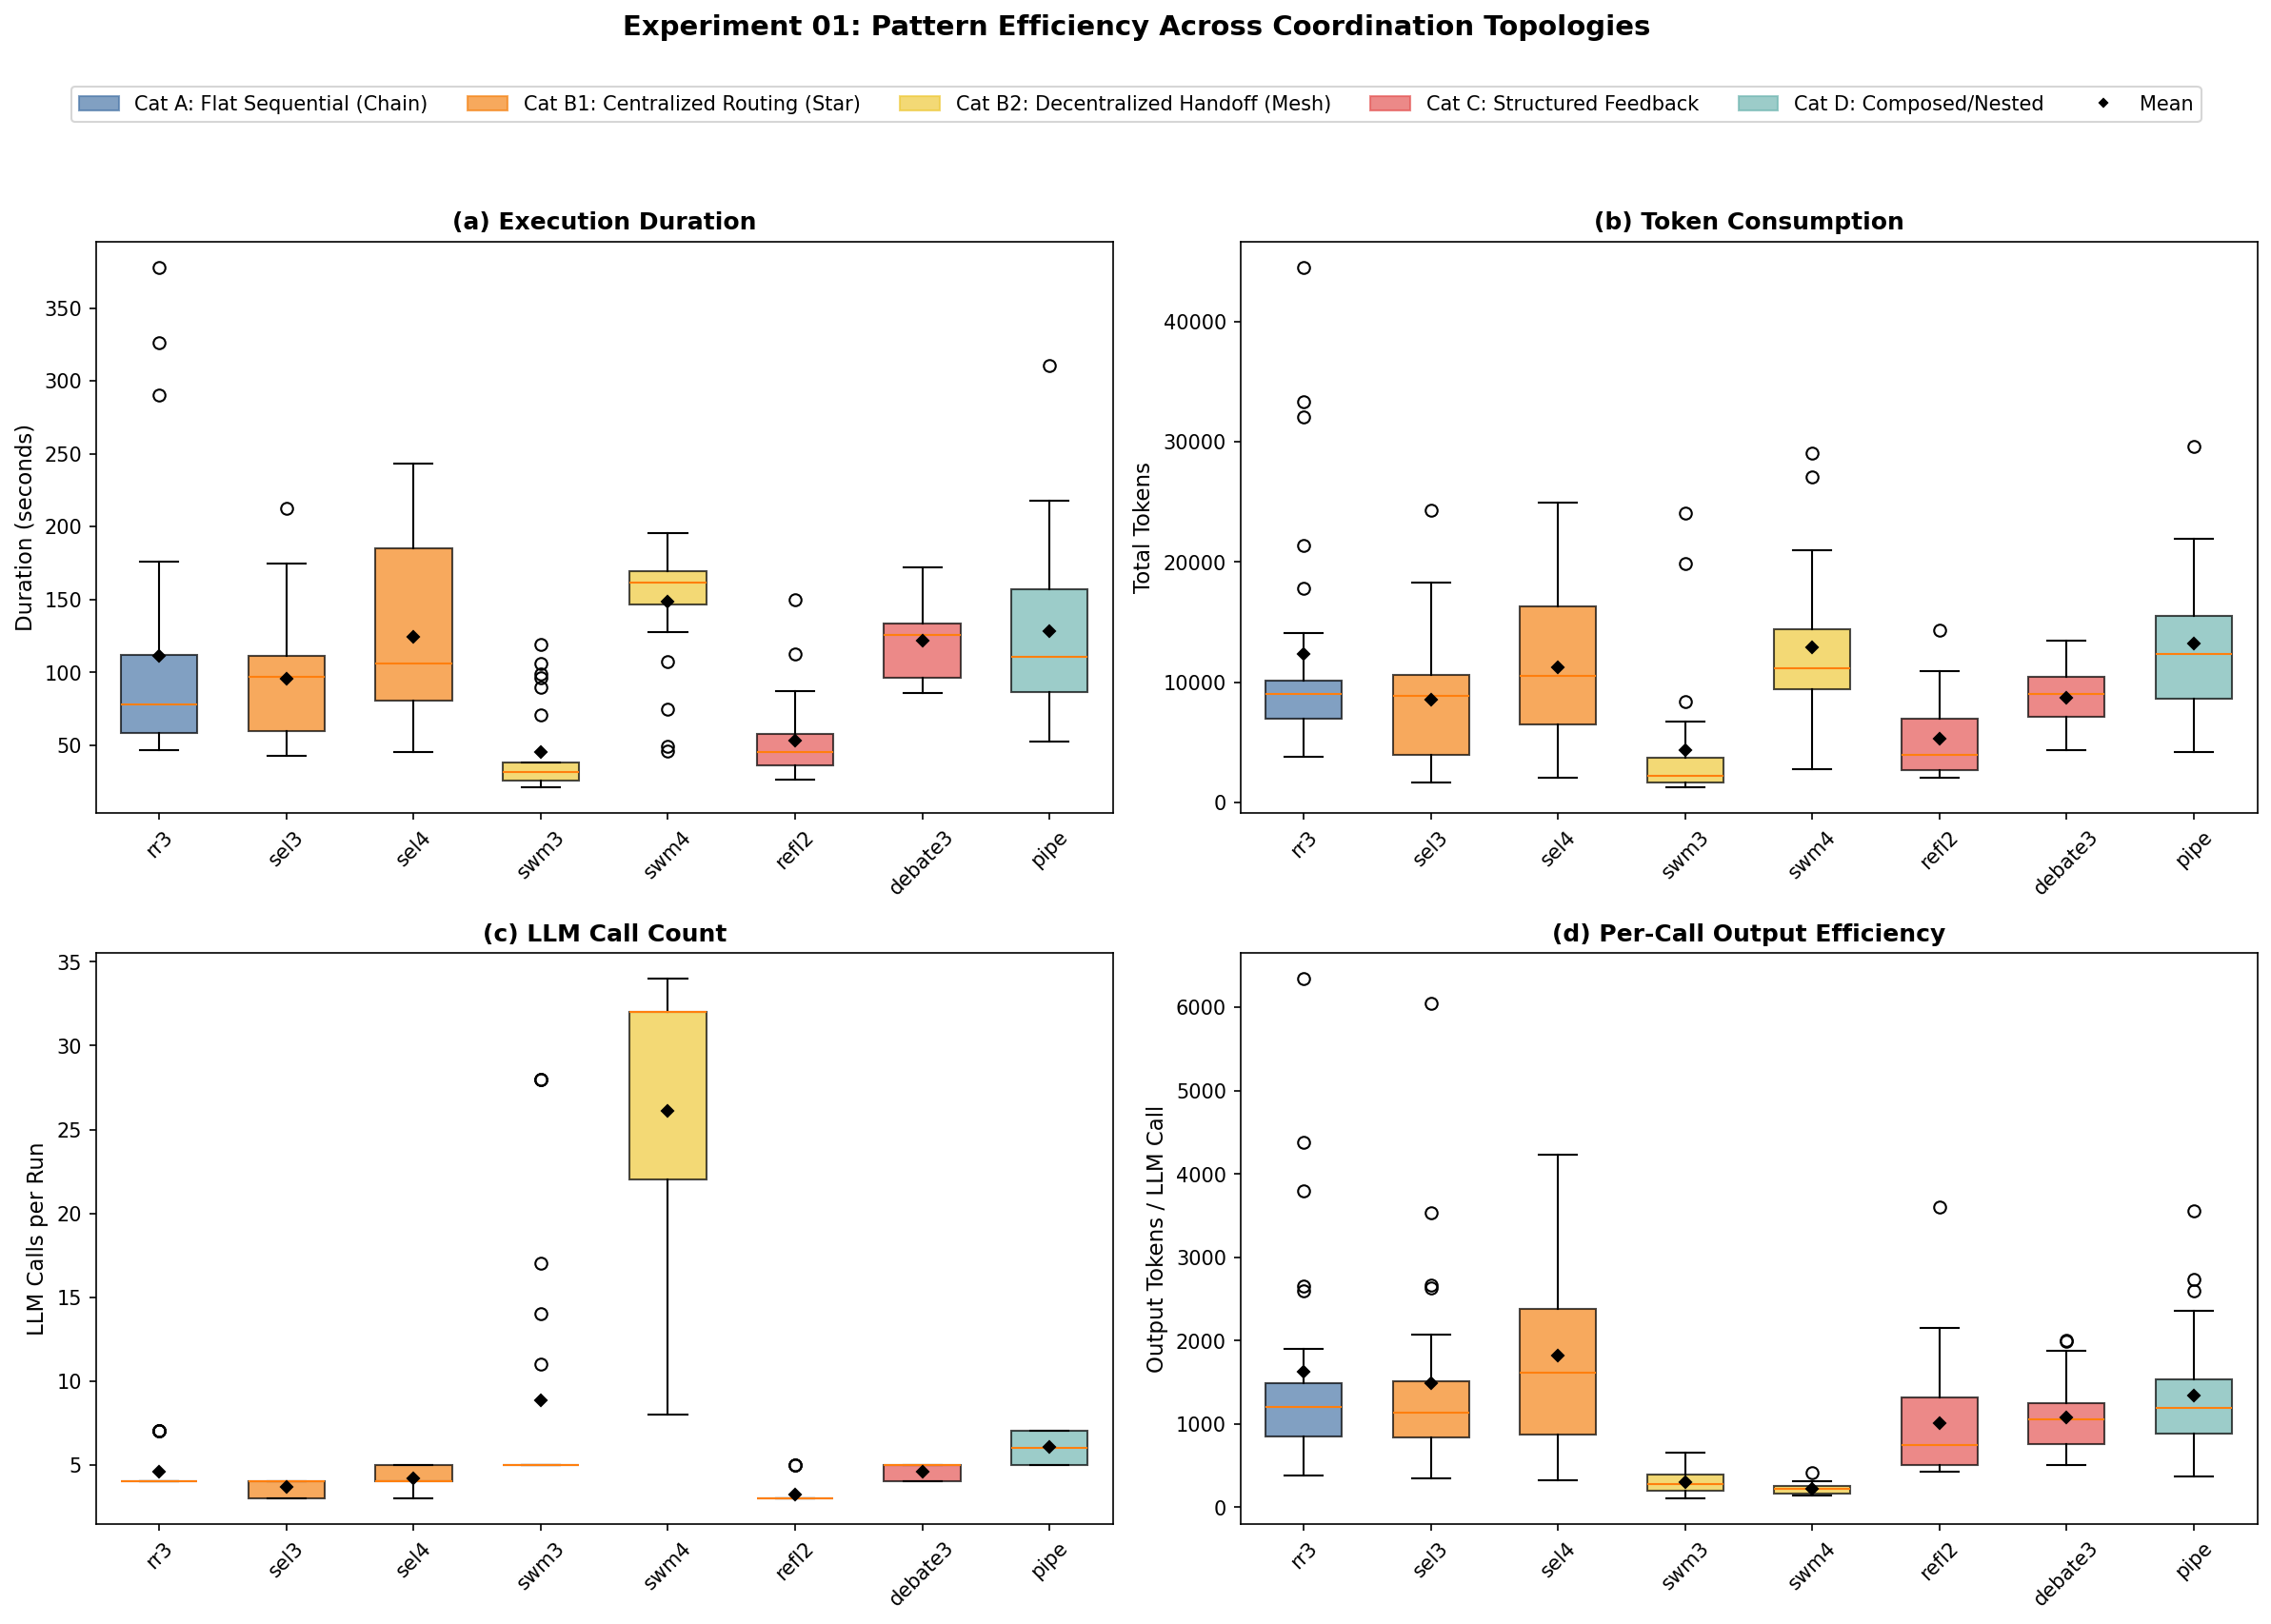
\includegraphics[width=\linewidth]{fig4_exp01_main.png}
\caption{Token consumption across 13 patterns by category. The 5.3$\times$ range from swm3 to MoA illustrates topology impact.}
\label{fig:exp01}
\end{figure}

\subsection{Experiment 02: Termination Quality (RQ2)}
\label{sec:exp02}

For five patterns, we apply G-Eval at each turn. \emph{Termination regret} $R = t_{\text{actual}} - t_{\text{optimal}}$ ranges from +0.2 (swm3) to +2.6 turns (rr3); quality loss spans 0.00 (refl2) to 0.65 (debate3) (Appendix Table~\ref{tab:regret}).

\paragraph{Finding 3: Three quality trajectory shapes.} (1)~rr3: \emph{plateau} after turn~3 ($Q$=4.5, loss=0.05). (2)~refl2: \emph{peak-at-turn-2} ($3.9 \to 4.8$, loss=0.00)---critic approval coincides with peak quality. (3)~debate3: \emph{monotonic decline} ($3.8 \to 3.3$, loss=0.65)---continued argumentation degrades output (Appendix Tables~\ref{tab:quality_traj}--\ref{tab:quality_dims}).

\paragraph{Implication.} The monotonic decline in debate quality challenges the intuition that more discussion improves outcomes. For practitioners, this means debate-style coordination should be limited to a single round unless a convergence monitor is deployed.

\paragraph{Finding 4: Regret varies 13$\times$ across topologies.} debate3 loses 0.65 quality from 2.0 excess turns; rr3 loses only 0.05 from 2.6 excess turns. Termination criteria must be topology-aware.

\paragraph{Finding 5: Reflection achieves highest quality with zero loss.} Refl2 attains $Q_{\text{peak}}$=4.80 (coherence 5.00, usefulness 4.95); its critic-approval mechanism closely approximates optimal stopping.

\paragraph{Evaluation Validation.} Six-model cross-validation from four providers (including open-weight Grok~3~Mini): $\kappa_w$=0.244 (GPT-4o-mini) to 0.507 (Opus~4.6); four exceed moderate threshold ($\geq$0.40). Bias splits across providers (strict: Haiku +0.91, GPT-5.4 +0.69, Opus +0.57; lenient: GPT-4o-mini $-$0.93, Gemini $-$0.82, Grok $-$0.60), confirming rank-order is evaluator-independent ($r$=0.43--0.66, all $p<0.01$; Appendix Table~\ref{tab:cross_val}).

\subsection{Experiment 03: Convergence Detection (RQ3)}
\label{sec:exp03}

\paragraph{Findings 6--7: Convergence signals are topology-dependent.} Sentence-BERT embeddings on 200 runs reveal that pipeline (D) exhibits the highest convergence rate (32.0\% at $\theta$=0.85), followed by centralized B1 (26.0\%). Feedback patterns (C) show 0\% convergence despite high mean cosine similarity (0.673), confirming they produce semantically similar but never-stabilizing content. Centralized routing shows the strongest positive trends (sel3: +0.397), while swm3 diverges ($-$0.560). Full analysis in Appendix Tables~\ref{tab:convergence}--\ref{tab:convergence_sensitivity}.

\subsection{Experiment 04: Error Attribution (RQ4)}
\label{sec:exp04}

\paragraph{Finding 8: Three distinct termination failure modes.} (1)~\emph{Context overflow} (Category~A): errors scale superlinearly with agent count (rr2=8.3\% $\to$ rr3=23.3\% $\to$ rr4=71.7\%). (2)~\emph{Turn explosion} (Category~B2): swm4 reaches max\_messages in 71.7\% of runs due to uncontrolled handoff chains. (3)~\emph{No failure} (B1, C, D except MoA): 100\% keyword termination. MoA always hits max\_messages because the aggregator does not emit \texttt{TERMINATE}. Factual tasks are error-immune while technical tasks produce 33.3\%$\to$100\% errors as system size increases (Appendix~\ref{app:errors}).

\subsection{Experiment 05: Adaptive Termination (RQ5)}
\label{sec:exp05}

We propose a \textbf{marginal utility stopping criterion}: $\Delta U(t) = \Delta Q(t) - \lambda \cdot \Delta C(t)$, where $\Delta Q$ is marginal quality gain, $\Delta C$ is marginal token cost (kilo-tokens), and $\lambda$ controls the tradeoff. The system stops when $\Delta U(t) \leq 0$. Unlike absolute utility which diverges to $-\infty$, marginal utility converges to zero via quality saturation. We test across 8 patterns, $\lambda \in \{0.0, 0.1, 0.5\}$, 25 tasks (800 runs).

\paragraph{Findings 9--11: $\Delta U$ is topology-dependent.} Patterns with reliable \texttt{TERMINATE} show minimal change (debate3: +8\%; pipe: +11\%), while swm4 (28\% keyword success) achieves \textbf{$-$65\% turns, $-$70\% tokens}. With $\lambda$=0: +131\% tokens; $\lambda \geq 0.1$: $-$13\% savings ($\lambda$-insensitive). As a \emph{replacement}, $\Delta U$ adds overhead for 7/8 patterns, confirming keyword near-optimality. This suggests complementary deployment.

\paragraph{Finding 12: Hybrid keyword+$\Delta U$ eliminates max\_messages failures across all categories.} Keyword+$\Delta U$ combined on six representative patterns spanning all categories ($\lambda$=0.1, 150 runs): swm4 (B2)---$\Delta U$ fires in 92\% of runs, achieving \textbf{78\% token savings} ($t$=$-$7.44, $p<$0.0001); debate3 (C)---keyword fires first in 64\%, 17\% savings ($p$=0.058). For keyword-reliable patterns, sel3 (B1) and pipe (D) show 100\% keyword termination with minor monitoring overhead ($-$5\% and $-$42\% respectively); rr3 (A) and refl2 (C) show 84\% keyword with $\Delta U$ as 16\% safety net and net savings of 24\% and 5\%. Zero max\_messages hits across all six patterns (Figure~\ref{fig:hybrid}).

\paragraph{Implication.} The asymmetric benefit of hybrid termination---dramatic for unreliable topologies, negligible or harmful for reliable ones---suggests a simple decision rule: deploy $\Delta U$ monitoring only when keyword termination success rate falls below 50\%.

\subsection{Cross-Model Validation}
\label{sec:cross_model}

\paragraph{Findings 13--14: Topology dynamics are model-invariant; routing efficiency is not.} GPT-4o-mini replication (200 runs, 8 patterns): cost ordering preserved ($\rho$=0.762, $p$=0.028). Absolute differences span 0.37--1.42$\times$ but \emph{relative} topology dynamics are model-invariant. GPT-4o-mini is more efficient at centralized routing (sel4: 0.37$\times$) but more verbose in chains (rr3: 1.42$\times$). Keyword reliability is model-dependent (swm4: GPT 25\% vs.\ Claude 28\%; Table~\ref{tab:cross_model}, Appendix).

\subsection{Experiment 06: Cost Prediction (RQ6)}
\label{sec:exp06}

\paragraph{Finding 15: Topology features predict 54\% of cost variance.} Using 718 runs, Random Forest achieves $R^2$=0.54 (5-fold CV) from pattern category, agent count, and task type. The interaction $\texttt{agents} \times \texttt{max\_msg}$ is the top predictor (importance=0.158). The remaining $\sim$46\% reflects task content complexity \citep{cohen1988}.

\paragraph{Finding 16: Holdout generalization is limited.} Exp05 holdout yields $R^2$=0.29; cross-distribution prediction requires task-level features.

\subsection{Experiment 07: Task Difficulty Interaction (RQ7)}
\label{sec:exp07}

We cross 5 patterns with 15 difficulty-graded tasks (5 domains $\times$ 3 levels) across 6 models (Haiku~4.5, Opus~4.6, GPT-4o-mini, GPT-5.4, Grok~3~Mini, Gemini-2.0-Flash), yielding 743 scored runs (3 repeats per cell for Haiku/GPT-4o-mini; 1 for others). Table~\ref{tab:difficulty} shows model-averaged quality (per-model: Table~\ref{tab:difficulty_6model}).

\begin{table}[t]
\centering
\caption{Difficulty $\times$ Pattern quality (6-model mean G-Eval overall). Bold = highest per row. Solo dominates easy for 5/6 models; Refl-2 leads medium/hard.}
\label{tab:difficulty}
{\small
\begin{tabular}{@{}lccccc@{}}
\toprule
& \textbf{Solo} & \textbf{Swm-3} & \textbf{Sel-3} & \textbf{Refl-2} & \textbf{Deb-3} \\
\midrule
\textbf{Easy} & \textbf{4.85} & 4.30 & 4.08 & 4.51 & 3.70 \\
\textbf{Med} & 3.52 & 3.39 & 3.24 & \textbf{3.77} & 2.84 \\
\textbf{Hard} & 3.04 & 2.96 & 3.00 & \textbf{3.27} & 2.67 \\
\bottomrule
\end{tabular}
}
\end{table}

\paragraph{Finding 17: Difficulty dominates pattern choice (6-model replication).} Across all 743 runs: difficulty main effect $H$=271.55, $p<$0.000001, $\eta^2_H$=0.364 (large); pattern main effect $H$=38.27, $p<$0.000001, $\eta^2_H$=0.046 (small). Difficulty explains \textbf{7.8$\times$} more variance than pattern choice. This dominance replicates in every individual model (all $p<$0.001). Pattern effects are significant within easy ($p<$0.001) and medium/hard ($p<$0.05) difficulty levels.

\paragraph{Finding 18: Solo dominance is model-invariant on easy; multi-agent benefit is capability-dependent.} Solo is best on easy tasks for \textbf{5/6 models} (GPT-5.4 ties with Refl-2 at 5.00). On medium tasks, Refl-2 outperforms solo for capable models---Haiku ($\Delta$=+0.67, $p$=0.003, $d$=1.26), GPT-5.4 ($\Delta$=+1.00, $p$=0.041, $d$=1.83), and Opus~4.6 ($\Delta$=+0.20)---but not for weaker models. On hard tasks, capability moderates: Opus ($\Delta$=+0.60), GPT-5.4, and Gemini benefit from Refl-2, while solo remains best for 3/6 models (Figure~\ref{fig:difficulty}).

\paragraph{Finding 19: Solo dominates cost-efficiency across models.} Solo achieves the highest quality-per-token ratio across difficulty levels, a pattern consistent across all 6 models. Even when Refl-2 achieves higher quality for capable models on medium/hard tasks, solo's substantially lower token cost preserves its cost-efficiency advantage.

\paragraph{Implication.} This result reframes the multi-agent design question: before selecting a coordination topology, practitioners should first assess whether the task difficulty warrants multi-agent coordination at all. For easy tasks, the answer is almost always no.

\begin{figure}[t]
\centering
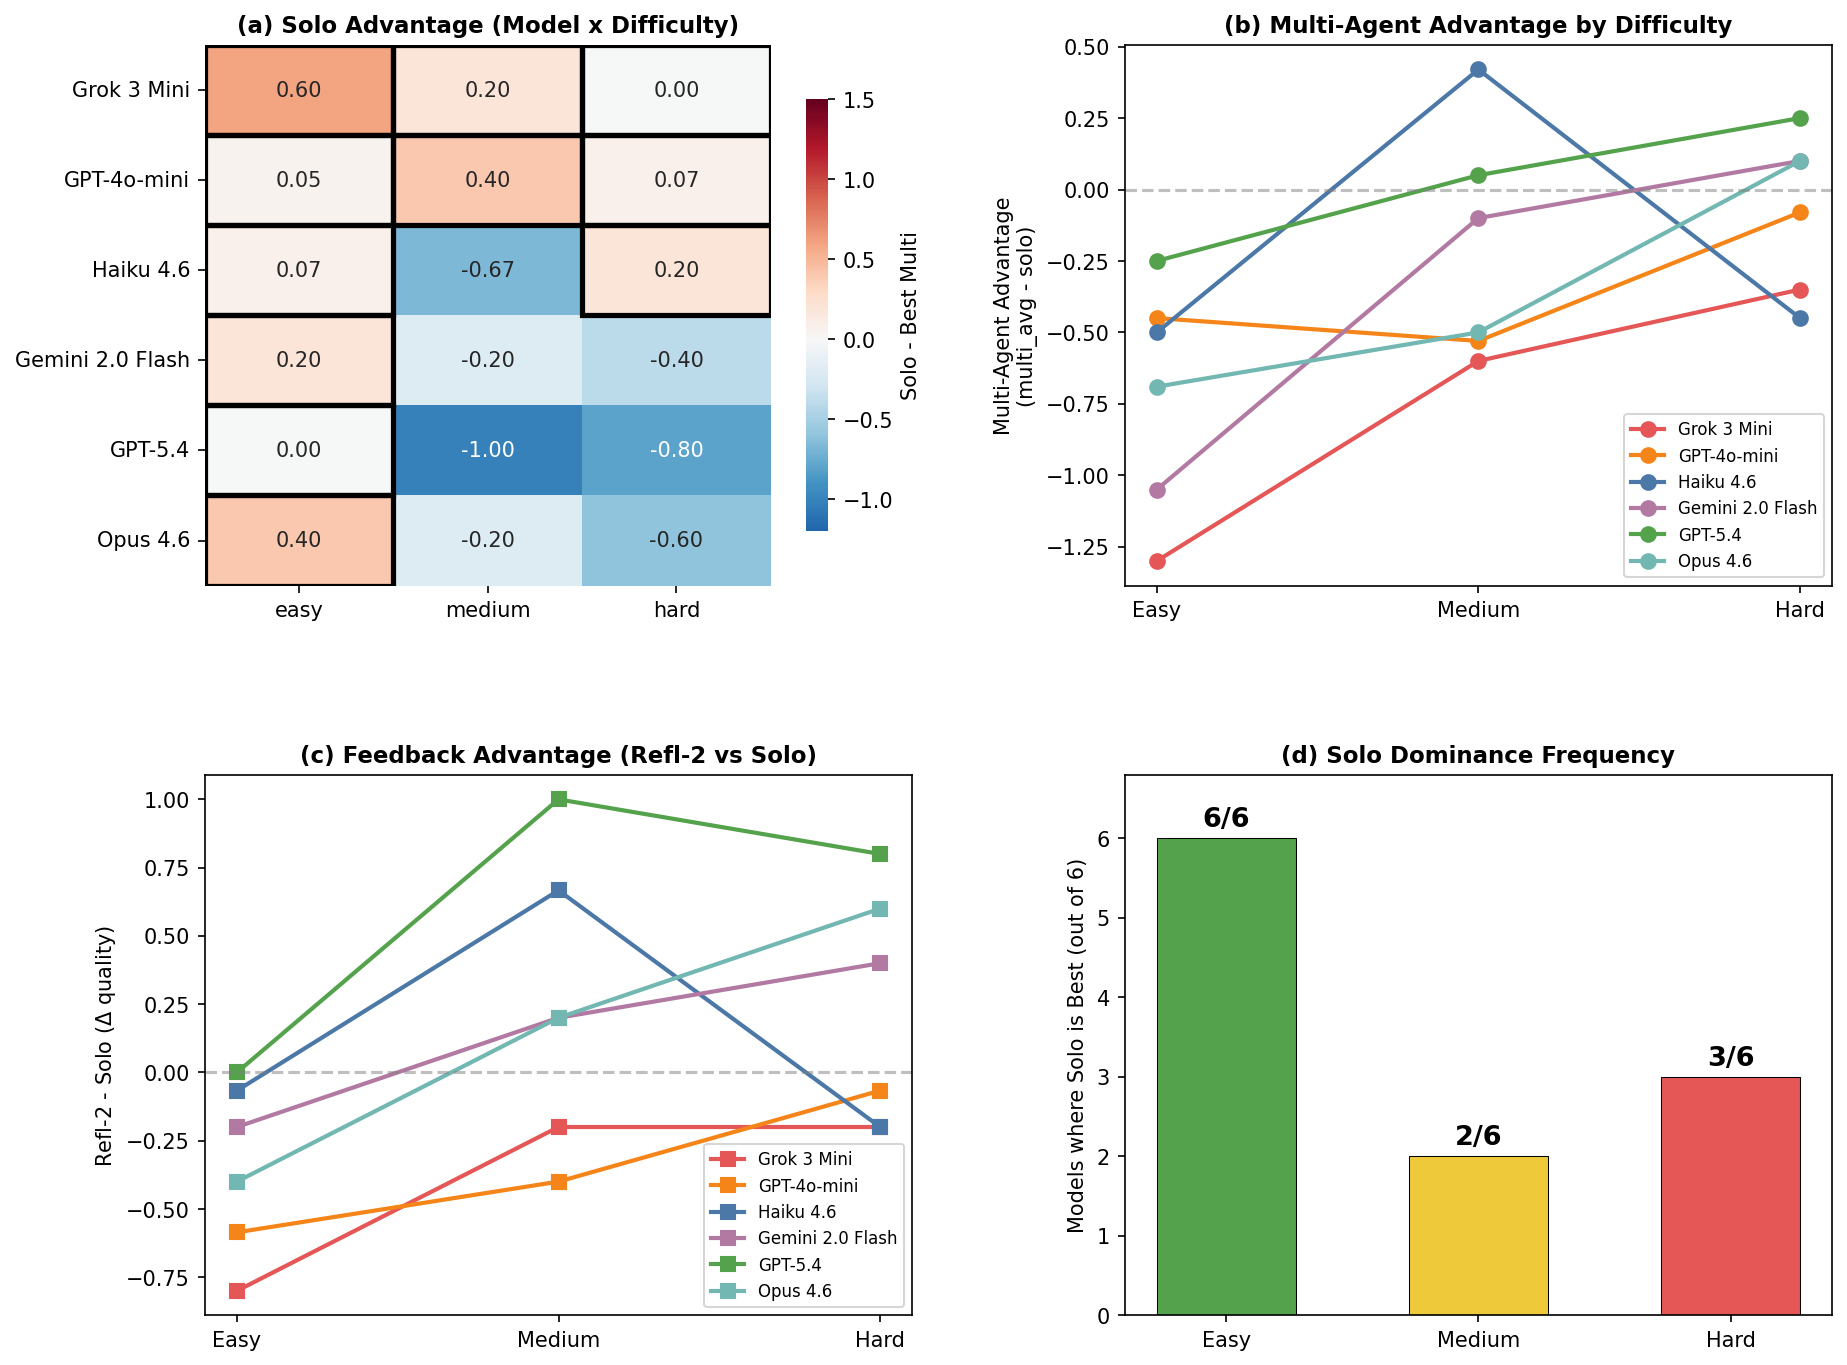
\includegraphics[width=\columnwidth]{fig10_difficulty_analysis.png}
\caption{Six-model difficulty $\times$ pattern analysis. (a)~Solo advantage heatmap: positive (red) = solo better; black border = solo is best pattern. (b)~Multi-agent advantage by difficulty per model. (c)~Refl-2 vs.\ Solo quality delta---inverted-U appears only for Haiku. (d)~Solo dominance frequency across models.}
\label{fig:difficulty}
\end{figure}

%=========================================================================
\vspace{-1mm}
\section{Discussion}
\label{sec:discussion}
\vspace{-1mm}
%=========================================================================

\subsection{Three Overturned Assumptions}
\vspace{-1mm}

Our results challenge three widely held assumptions in multi-agent system design:

\textbf{(1)~``More agents = more cost'' is false.} swm3 (3 agents) is 12\% cheaper than rr2 (2 agents) because routing strategy---not headcount---drives token consumption (Finding~2). Practitioners who avoid multi-agent setups purely for cost reasons may miss efficient configurations.

\textbf{(2)~``More rounds = better quality'' is false.} Debate quality declines monotonically after round~1 (Finding~3), and termination regret varies 13$\times$ across topologies (Finding~4). The intuition that continued deliberation refines output is actively harmful for debate topologies.

\textbf{(3)~``Topology is the key design decision'' is false.} Task difficulty explains 7.8$\times$ more quality variance than pattern choice (Finding~17). The primary optimization target is not \emph{which} topology to deploy but \emph{whether} multi-agent coordination is warranted at all.

\subsection{Design Guidelines}
\vspace{-1mm}

\textbf{G1.}~Match termination to topology: sequential uses $2n$ max\_messages; feedback monitors convergence; composed applies per-stage termination.
\textbf{G2.}~Budget for superlinear input growth ($O(n \cdot k \cdot L)$); use context summarization.
\textbf{G3.}~Consider task-topology interaction: cost varies 2.2$\times$ across task categories; debate3 is domain-invariant (CV=0.14), swm3 domain-sensitive (CV=0.67).
\textbf{G4.}~Deploy hybrid keyword+$\Delta U$ termination for topologies with $<$50\% keyword reliability (e.g., swm4: 28\%), recovering up to 78\% of wasted tokens; retain keyword-only for reliable topologies (sel, pipe, refl) to avoid monitoring overhead.
\textbf{G5.}~Match complexity to difficulty: decide \emph{whether} before \emph{which}---solo for easy tasks (5/6 models); Refl-2 for medium/hard only with capable base models.

\subsection{Limitations}
\vspace{-1mm}

\begin{enumerate}
\item \textbf{Model coverage}: six models from four providers (743 runs), including one open-weight model (Grok~3~Mini, Apache~2.0); extension to additional open-weight families (Llama, Mistral) remains future work. Key findings---difficulty dominance ($\eta^2_H$=0.364) and solo optimality on easy tasks---replicate across all six models (Section~\ref{sec:exp07}), and topology cost ordering is preserved under GPT-4o-mini ($\rho$=0.762, $p$=0.028).
\item \textbf{Task suite}: 25 tasks across 9 domains; excludes interactive and multi-modal tasks. Standard benchmarks (e.g., MMLU, HumanEval) target single-correct-answer evaluation and cannot capture the per-turn quality trajectories central to termination analysis; our suite is designed for this purpose.
\item \textbf{Quality estimator}: $\kappa_w$=0.244--0.507 with bidirectional bias across providers; single expert evaluator. However, rank-order agreement is significant across all six cross-validators ($r$=0.43--0.66, all $p<$0.01; four exceed moderate threshold $\kappa_w \geq 0.40$), and the bidirectional bias pattern (three lenient, three strict) argues against systematic evaluator bias.
\item \textbf{Hybrid termination}: validated on six patterns across four categories (150 runs); extension to all 14 patterns remains future work.
\item \textbf{Cost proxy}: token count ignores latency and dollar costs; per-pattern $n$=25--60.
\end{enumerate}

%=========================================================================
\vspace{-1mm}
\section{Conclusion}
\label{sec:conclusion}
\vspace{-1mm}
%=========================================================================

Through 2,200+ runs across 14 topologies and six models from four providers (including open-weight Grok~3~Mini), we establish five key results. \textbf{(1)~Topology determines termination}: overhead spans 3.3--17.4$\times$ with fundamentally different scaling for centralized vs.\ decentralized routing. \textbf{(2)~More agents can cost less}: swm3 (3 agents) beats rr2 (2 agents) by 12\%. \textbf{(3)~Simple heuristics work---almost}: keyword is near-optimal for 7/8 topologies; hybrid keyword+$\Delta U$ achieves 78\% savings for the exception (150 runs across six patterns, zero max\_messages hits). \textbf{(4)~Difficulty trumps topology}: $\eta^2_H$=0.364 vs.\ 0.046; solo is best on easy tasks for 5/6 models; Refl-2 benefits capable models on medium/hard ($d$=1.26--1.83). \textbf{(5)~Decide \emph{whether} before \emph{which}}: the primary optimization target is not topology selection but the difficulty-conditioned decision of whether to use multi-agent coordination at all. We release our framework and five topology-aware design guidelines.

\section*{Reproducibility Statement}

All experiments use publicly available frameworks (AutoGen) with fully specified configurations (pattern definitions, task prompts, and hyperparameters) provided in the supplementary materials. We report exact model versions, random seeds, and repeat counts for all experiments. Statistical tests include effect sizes and confidence intervals throughout. Code and data will be released upon acceptance.

\paragraph{LLM Disclosure.} Per COLM policy, we disclose the following LLM usage in this research: (1)~Claude Haiku~4.5 as the base agent model for Experiments~01--06; (2)~Claude Opus~4.6, GPT-4o-mini, GPT-5.4, Grok~3~Mini (open-weight, Apache~2.0), and Gemini~2.0~Flash as additional agent models for cross-model validation (Experiment~07); (3)~Claude Sonnet~4.5 as the G-Eval judge model for quality scoring. LLMs were not used to originate research ideas or generate paper content.

%=========================================================================
% References
%=========================================================================

\bibliography{references}
\bibliographystyle{colm2026_conference}

%=========================================================================
\appendix
%=========================================================================

\section{Related Work Comparison}
\label{app:related_table}

\begin{table}[H]
\centering
\caption{Comparison with related work on multi-agent termination.}
\label{tab:related}
{\small
\begin{tabular}{@{}lcccc@{}}
\toprule
\textbf{Work} & \textbf{Patterns} & \textbf{Categories} & \textbf{Adaptive} & \textbf{Convergence} \\
\midrule
MAST (NeurIPS '25) & 2 & Debate, voting & No & Trajectory \\
REFRAIN ('25) & 1 & CoT (1-agent) & Yes & N/A \\
\citet{hu2025when} & 1 & Debate & Yes & Distribution \\
Aegean ('25) & N/A & Consensus & Yes & Quorum \\
\citet{cemri2025why} & $\sim$5 & Mixed & No & Post-hoc \\
G-Designer (ICML '25) & Dynamic & GNN-gen. & No & N/A \\
Scaling Agents ('25) & 5 & 4 types & No & N/A \\
\citet{wang2025rethinking} & 1 & Debate & No & Semantic \\
AgentDropout (ACL '25) & Variable & Comm.\ graphs & No & N/A \\
SupervisorAgent ('25) & 1+ & Runtime sup. & Yes & Context \\
AgentsNet ('25) & Variable & Graph coord. & No & N/A \\
MultiAgentBench ('25) & Variable & Collab/comp. & No & N/A \\
\midrule
\textbf{Ours} & \textbf{14} & \textbf{6 categories} & \textbf{Yes} & \textbf{Claim-level} \\
\bottomrule
\end{tabular}
}
\end{table}

\section{Task Suite}
\label{app:tasks}

\begin{table*}[t]
\centering
\caption{Complete task suite (25 tasks across 9 domains and 4 cognitive types).}
\label{tab:tasks}
\resizebox{\textwidth}{!}{
\begin{tabular}{@{}llllp{10cm}@{}}
\toprule
\textbf{ID} & \textbf{Domain} & \textbf{Type} & \textbf{Diff.} & \textbf{Task Description} \\
\midrule
sci\_01 & Science & Factual & Med & Explain the three laws of thermodynamics and their practical engineering implications \\
sci\_02 & Science & Analytical & Med & Describe photosynthesis including light-dependent/independent reactions; compare C3, C4, CAM pathways \\
sci\_03 & Science & Creative & Hard & Propose three novel experimental approaches to detect dark matter with theoretical motivation \\
cs\_01 & CS & Factual & Med & Explain the TCP/IP protocol stack layers and data flow from application to physical layer \\
cs\_02 & CS & Technical & Med & Implement an LRU cache with O(1) get/put operations; explain data structure choices \\
cs\_03 & CS & Analytical & Med & Compare microservices vs.\ monolithic architecture for 100K DAU e-commerce \\
hist\_01 & History & Factual & Med & Analyze the main causes of World War I (political, economic, social factors) \\
hist\_02 & History & Analytical & Hard & Compare the fall of the Roman Empire with the decline of the British Empire \\
hist\_03 & History & Creative & Hard & Alternate history: What if the printing press was invented in Song Dynasty China? \\
phil\_01 & Philosophy & Factual & Med & Explain Kant's categorical imperative vs.\ Mill's utilitarianism on moral decision-making \\
phil\_02 & Philosophy & Analytical & Med & Analyze the trolley problem variants across deontological, utilitarian, virtue ethics \\
phil\_03 & Philosophy & Creative & Hard & Design a thought experiment challenging personal identity in the age of AI mind uploading \\
law\_01 & Law/Pol. & Factual & Med & Explain separation of powers in presidential vs.\ parliamentary systems \\
law\_02 & Law/Pol. & Analytical & Hard & Analyze AI-generated content in copyright law: EU AI Act, US fair use, Korean approaches \\
law\_03 & Law/Pol. & Creative & Hard & Draft a policy proposal for regulating autonomous vehicles (liability, insurance, testing) \\
game\_01 & Gaming & Factual & Med & Explain game design principles: feedback loops, flow state, MDA framework \\
game\_02 & Gaming & Technical & Hard & Design real-time multiplayer matchmaking (ELO/Glicko, latency, queue balancing) \\
game\_03 & Gaming & Creative & Hard & Design a game teaching quantum computing through puzzle mechanics \\
eng\_01 & Engineering & Factual & Med & Explain structural load analysis for bridges (dead, live, wind, seismic loads) \\
eng\_02 & Engineering & Technical & Hard & Design a water treatment plant for 200K people (stages, capacity, standards) \\
eng\_03 & Engineering & Analytical & Med & Compare traditional vs.\ 3D-printed construction for affordable housing \\
biz\_01 & Business & Creative & Hard & Create a business plan for an AI-powered K-12 education startup \\
biz\_02 & Business & Analytical & Med & Compare VC funding vs.\ bootstrapping for B2B SaaS startups \\
biz\_03 & Business & Analytical & Hard & Evaluate EV market entry strategy for Southeast Asia \\
med\_01 & Medicine & Analytical & Hard & Compare mRNA vs.\ protein subunit vaccines for pandemic preparedness \\
\bottomrule
\end{tabular}
}
\end{table*}

\section{Detailed Results}
\label{app:results}

\subsection{Category A: Flat Sequential Patterns}

\begin{table}[H]
\centering
\caption{Category A efficiency metrics (successful runs only).}
\label{tab:catA}
{\small
\begin{tabular}{@{}lrrr@{}}
\toprule
\textbf{Metric} & \textbf{rr2} ($n$=2) & \textbf{rr3} ($n$=3) & \textbf{Ratio} \\
\midrule
Successful runs & 55/60 & 46/60 & -- \\
Error rate & 8.3\% & 23.3\% & 2.81$\times$ \\
Mean LLM calls & 2.0 & 3.5 & 1.75$\times$ \\
Mean duration (s) & 52.4 & 96.6 & 1.84$\times$ \\
Mean tokens (in) & 1,594 & 4,132 & 2.59$\times$ \\
Mean tokens (out) & 3,165 & 5,989 & 1.89$\times$ \\
Mean total tokens & 4,759 & 10,121 & 2.13$\times$ \\
Output tokens/call & 1,583 & 1,711 & 1.08$\times$ \\
\bottomrule
\end{tabular}
}
\end{table}

\begin{table}[H]
\centering
\caption{Full 3-pattern comparison for Category A (successful runs only).}
\label{tab:catA_full}
{\small
\begin{tabular}{@{}lrrrrr@{}}
\toprule
\textbf{Metric} & \textbf{rr2} & \textbf{rr3} & \textbf{rr4} & \textbf{rr3/rr2} & \textbf{rr4/rr2} \\
\midrule
Successful & 55/60 & 46/60 & 17/60 & -- & -- \\
Error rate & 8.3\% & 23.3\% & 71.7\% & 2.81$\times$ & 8.64$\times$ \\
Duration (s) & 52.4 & 96.6 & 118.8 & 1.84$\times$ & 2.27$\times$ \\
Tokens (in) & 1,594 & 4,132 & 4,274 & 2.59$\times$ & 2.68$\times$ \\
Tokens (out) & 3,165 & 5,989 & 7,767 & 1.89$\times$ & 2.45$\times$ \\
Total tokens & 4,759 & 10,121 & 12,040 & 2.13$\times$ & 2.53$\times$ \\
Out/agent turn & 1,583 & 1,701 & 1,942 & 1.07$\times$ & 1.23$\times$ \\
\bottomrule
\end{tabular}
}
\end{table}

\begin{table}[H]
\centering
\caption{Task category effects (Categories A combined).}
\label{tab:task_effects}
{\small
\begin{tabular}{@{}lrrrrl@{}}
\toprule
\textbf{Task Cat.} & \textbf{Runs} & \textbf{Dur.(s)} & \textbf{Tokens} & \textbf{Err.\%} & \textbf{Character.} \\
\midrule
Factual & 30 & 66.5 & 6,183 & 0\% & Retrieval, short \\
Creative & 30 & 93.3 & 8,578 & 10.0\% & Open-ended \\
Analytical & 30 & 82.1 & 8,152 & 10.0\% & Structured \\
Technical & 19 & 61.9 & 9,100 & 42.1\% & Token-dense \\
\bottomrule
\end{tabular}
}
\end{table}

\subsection{Category B: Dynamic Routing Patterns}

\begin{table}[H]
\centering
\caption{Category B efficiency metrics (all runs successful).}
\label{tab:catB}
{\small
\begin{tabular}{@{}lrrrr@{}}
\toprule
\textbf{Metric} & \textbf{Sel-3} & \textbf{Sel-4} & \textbf{Swm-3} & \textbf{Swm-4} \\
\midrule
Runs & 60/60 & 60/60 & 60/60 & 60/60 \\
Duration (s) & 115.2 & 161.9 & 75.2 & 185.0 \\
Tokens (in) & 2,076 & 2,457 & 1,364 & 6,786 \\
Tokens (out) & 5,775 & 9,138 & 2,833 & 6,535 \\
Total tokens & 7,851 & 11,595 & 4,196 & 13,321 \\
Turns & 3.5 & 4.1 & 10.2 & 25.0 \\
Agent turns & 2.5 & 3.1 & 9.2 & 24.0 \\
Out/agent turn & 2,114 & 2,616 & 337 & 330 \\
\bottomrule
\end{tabular}
}
\end{table}

\begin{table}[H]
\centering
\caption{Cross-strategy comparison (Category A vs.\ B).}
\label{tab:cross_AB}
{\small
\begin{tabular}{@{}lcrrrr@{}}
\toprule
\textbf{Pattern} & \textbf{Agents} & \textbf{Dur.(s)} & \textbf{Tokens} & \textbf{vs rr3 Dur.} & \textbf{vs rr3 Tok.} \\
\midrule
rr2 & 2 & 52.4 & 4,759 & 0.54$\times$ & 0.47$\times$ \\
rr3 & 3 & 96.6 & 10,121 & 1.00$\times$ & 1.00$\times$ \\
sel3 & 3+1 & 115.2 & 7,851 & 1.19$\times$ & 0.78$\times$ \\
sel4 & 4+1 & 161.9 & 11,595 & 1.68$\times$ & 1.15$\times$ \\
swm3 & 3 & 75.2 & 4,196 & 0.78$\times$ & 0.41$\times$ \\
swm4 & 4 & 185.0 & 13,321 & 1.92$\times$ & 1.32$\times$ \\
\bottomrule
\end{tabular}
}
\end{table}

\subsection{Category C: Structured Feedback Patterns}

\begin{table}[H]
\centering
\caption{Category C efficiency metrics (all runs successful).}
\label{tab:catC}
{\small
\begin{tabular}{@{}lrrrr@{}}
\toprule
\textbf{Metric} & \textbf{Refl-2} & \textbf{Refl-3} & \textbf{Deb-3} & \textbf{Deb-4} \\
\midrule
Runs & 60/60 & 60/60 & 60/60 & 60/60 \\
Duration (s) & 60.2 & 120.2 & 156.6 & 180.9 \\
Tokens (in) & 1,485 & 3,343 & 3,480 & 5,217 \\
Tokens (out) & 3,752 & 8,752 & 5,834 & 6,420 \\
Total tokens & 5,237 & 12,095 & 9,313 & 11,637 \\
Turns & 3.2 & 4.5 & 4.5 & 5.4 \\
Agent turns & 2.2 & 3.5 & 3.5 & 4.4 \\
Out/agent turn & 1,732 & 2,537 & 1,691 & 1,448 \\
\bottomrule
\end{tabular}
}
\end{table}

\subsection{Category D: Composed Patterns}

\begin{table}[H]
\centering
\caption{Category D efficiency metrics (all runs successful).}
\label{tab:catD}
{\small
\begin{tabular}{@{}lrr@{}}
\toprule
\textbf{Metric} & \textbf{Pipe} ($n$=5) & \textbf{MoA} ($n$=4) \\
\midrule
Runs & 60/60 & 60/60 \\
Duration (s) & 129.6 & 103.0 \\
Tokens (in) & 4,275 & 4,875 \\
Tokens (out) & 9,581 & 17,458 \\
Total tokens & 13,856 & 22,333 \\
Turns & 6.0 & 11.0 \\
Agent turns & 4.0 & 7.0 \\
Out/agent turn & 2,325 & 2,494 \\
\bottomrule
\end{tabular}
}
\end{table}

\begin{table}[H]
\centering
\caption{Category D task breakdown (total tokens by task category).}
\label{tab:catD_tasks}
{\small
\begin{tabular}{@{}lrrr@{}}
\toprule
\textbf{Task Cat.} & \textbf{Pipe} & \textbf{MoA} & \textbf{MoA/Pipe} \\
\midrule
Factual & 9,930 & 15,064 & 1.52$\times$ \\
Creative & 13,929 & 17,826 & 1.28$\times$ \\
Analytical & 12,342 & 18,598 & 1.51$\times$ \\
Technical & 19,223 & 37,844 & 1.97$\times$ \\
Tech/Fact ratio & 1.94$\times$ & 2.51$\times$ & -- \\
\bottomrule
\end{tabular}
}
\end{table}

\subsection{Statistical Tests}

\begin{table}[H]
\centering
\caption{Kruskal-Wallis tests across 5 categories (df=4, $N$=718).}
\label{tab:kruskal}
{\small
\begin{tabular}{@{}lrrl@{}}
\toprule
\textbf{Metric} & \textbf{$H$} & \textbf{$p$-value} & \textbf{Sig.} \\
\midrule
Turn count & 408.606 & $<$0.001 & Yes \\
Duration (s) & 70.776 & $<$0.001 & Yes \\
Total tokens & 132.333 & $<$0.001 & Yes \\
Input tokens & 60.885 & $<$0.001 & Yes \\
Output tokens & 120.565 & $<$0.001 & Yes \\
\bottomrule
\end{tabular}
}
\end{table}

\begin{table}[H]
\centering
\caption{Pairwise Mann-Whitney U tests for total tokens.}
\label{tab:pairwise}
{\small
\begin{tabular}{@{}lrrl@{}}
\toprule
\textbf{Comparison} & \textbf{$U$} & \textbf{$p$-value} & \textbf{Sig.} \\
\midrule
A vs B1 & 6,000 & 0.042 & * \\
A vs B2 & 7,176 & 0.857 & No \\
A vs C & 11,034 & $<$0.001 & *** \\
A vs D & 1,778 & $<$0.001 & *** \\
B1 vs B2 & 8,157 & 0.075 & No \\
B1 vs C & 14,035 & 0.695 & No \\
B1 vs D & 3,010 & $<$0.001 & *** \\
B2 vs C & 12,348 & 0.028 & * \\
B2 vs D & 2,944 & $<$0.001 & *** \\
C vs D & 5,216 & $<$0.001 & *** \\
\bottomrule
\end{tabular}
}
\end{table}

\begin{table}[H]
\centering
\caption{Token consumption by category.}
\label{tab:category_tokens}
{\small
\begin{tabular}{@{}lrrr@{}}
\toprule
\textbf{Category} & \textbf{Median} & \textbf{Mean} & $N$ \\
\midrule
A (Chain) & 7,420 & 7,898 & 118 \\
B1 (Centralized Routing) & 9,197 & 9,723 & 120 \\
B2 (Decentralized Handoff) & 9,142 & 8,759 & 120 \\
C (Structured Feedback) & 9,247 & 9,571 & 240 \\
D (Composed/Nested) & 15,865 & 18,094 & 120 \\
\bottomrule
\end{tabular}
}
\end{table}

\subsection{Quality Trajectories}

\begin{table}[H]
\centering
\caption{Quality trajectories (mean overall score by substantive turn).}
\label{tab:quality_traj}
{\small
\begin{tabular}{@{}lcccccc@{}}
\toprule
\textbf{Pattern} & $t_1$ & $t_2$ & $t_3$ & $t_4$ & $t_5$ & $t_6$ \\
\midrule
rr3 & 3.9 & 4.2 & 4.5 & 4.1 & 4.1 & 4.1 \\
sel3 & 3.8 & 3.5 & 2.7 & 4.0 & 4.0 & -- \\
swm3 & 4.2 & 3.0 & 2.0 & -- & -- & -- \\
refl2 & 3.9 & 4.8 & 4.0 & 4.0 & -- & -- \\
debate3 & 3.8 & 3.4 & 3.3 & 3.3 & -- & -- \\
\bottomrule
\end{tabular}
}
\end{table}

\begin{table}[H]
\centering
\caption{Quality dimension breakdown (final turn averages).}
\label{tab:quality_dims}
{\small
\begin{tabular}{@{}lccccc@{}}
\toprule
\textbf{Pattern} & \textbf{Acc.} & \textbf{Compl.} & \textbf{Coh.} & \textbf{Useful.} & \textbf{Overall} \\
\midrule
refl2 & 4.80 & 4.25 & 5.00 & 4.95 & 4.80 \\
rr3 & 4.50 & 3.75 & 4.25 & 4.70 & 4.45 \\
swm3 & 4.25 & 3.80 & 4.45 & 4.35 & 4.05 \\
sel3 & 3.85 & 3.15 & 3.35 & 3.80 & 3.40 \\
debate3 & 3.75 & 2.70 & 3.35 & 3.55 & 3.35 \\
\bottomrule
\end{tabular}
}
\end{table}

\subsection{Cross-Validation}

\begin{table}[H]
\centering
\caption{Cross-model agreement (overall dimension): Claude G-Eval vs.\ six independent models from four provider families.}
\label{tab:cross_val}
{\small
\begin{tabular}{@{}llccccc@{}}
\toprule
\textbf{Cross-Validator} & \textbf{Provider} & $N$ & $r$ & $\rho$ & $\kappa_w$ & $\Delta$ \\
\midrule
GPT-4o-mini & OpenAI & 40 & 0.434 & 0.389 & 0.244 & $-$0.93 \\
Gemini 2.0 Flash & Google & 100 & 0.569 & 0.500 & 0.359 & $-$0.82 \\
GPT-5.4 & OpenAI & 100 & 0.540 & 0.525 & \textbf{0.415} & +0.69 \\
Haiku 4.5 & Anthropic & 100 & 0.662 & 0.650 & \textbf{0.425} & +0.91 \\
Grok 3 Mini & xAI & 100 & 0.628 & 0.626 & \textbf{0.449} & $-$0.60 \\
Opus 4.6 & Anthropic & 100 & 0.632 & 0.649 & \textbf{0.507} & +0.57 \\
\bottomrule
\end{tabular}
}
\end{table}

\begin{figure}[H]
\centering
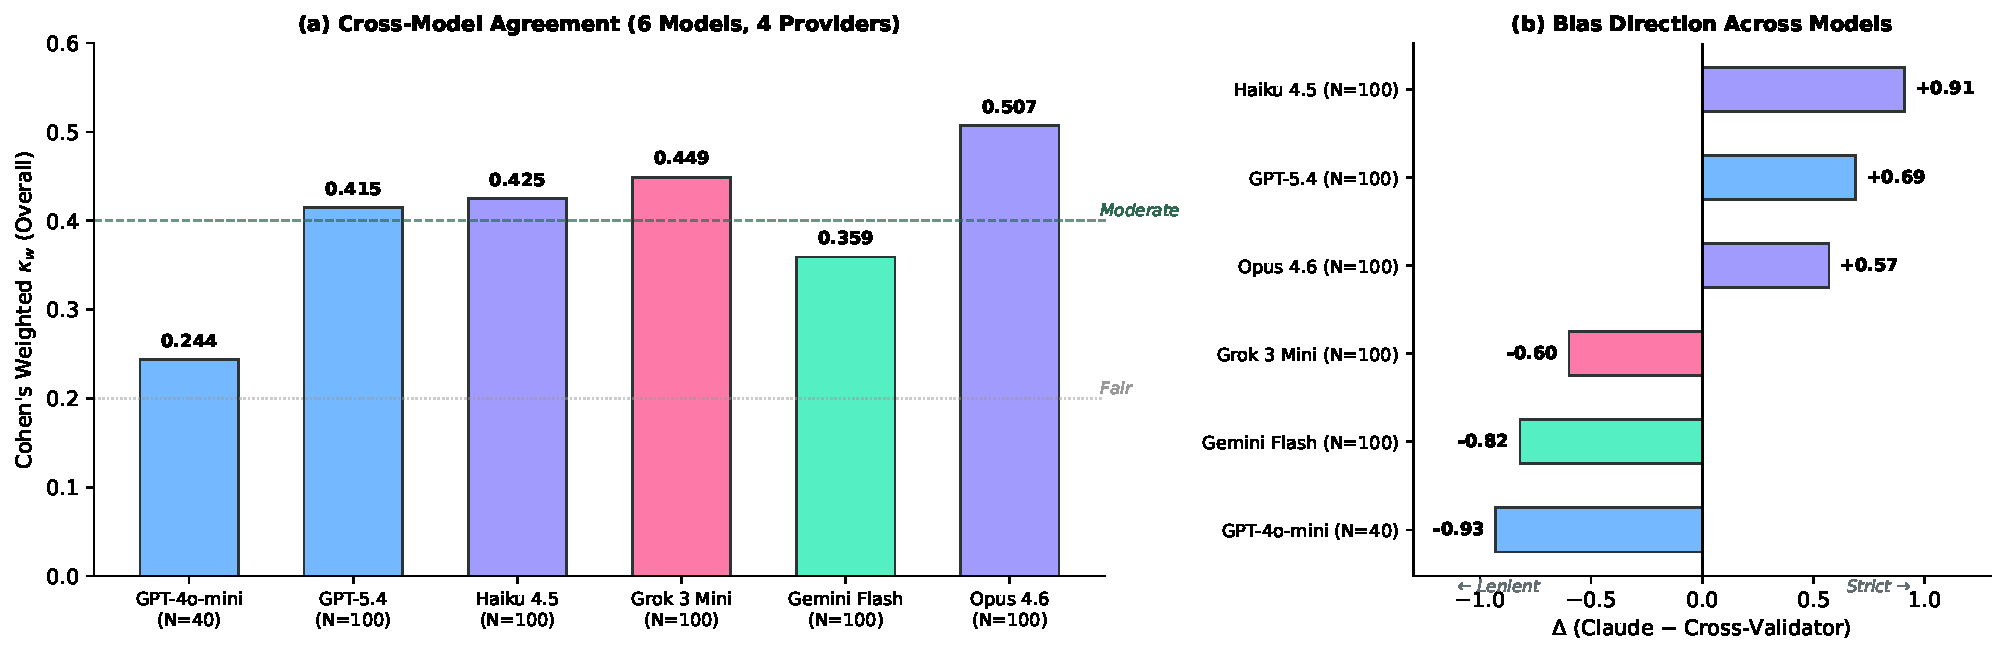
\includegraphics[width=\linewidth]{fig_kappa_comparison.pdf}
\caption{Cross-model evaluation validation across six models from four providers. (a)~Overall Cohen's $\kappa_w$: four of six models (GPT-5.4, Haiku~4.5, Grok~3~Mini, Opus~4.6) cross the ``moderate'' threshold (0.40), with Opus achieving the highest $\kappa_w$=0.507. (b)~Bias direction splits across providers: strict (Haiku $\Delta$=+0.91, GPT-5.4 $\Delta$=+0.69, Opus $\Delta$=+0.57) vs.\ lenient (GPT-4o-mini $\Delta$=$-$0.93, Gemini $\Delta$=$-$0.82, Grok $\Delta$=$-$0.60), confirming rank-ordering is evaluator-independent.}
\label{fig:kappa}
\end{figure}

\subsection{Marginal Utility Pre-Validation}

\begin{table}[H]
\centering
\caption{Marginal utility convergence analysis ($\lambda$=0.1, from exp02 data).}
\label{tab:prevalidation}
{\small
\begin{tabular}{@{}llccccccc@{}}
\toprule
\textbf{Pattern} & \textbf{Cat.} & $t_{\Delta U \leq 0}$ & $t_{\text{opt}}$ & $t_{\text{act}}$ & $Q_{\text{opt}}$ & $Q_{\text{act}}$ & $Q_{\text{loss}}$ & Regret \\
\midrule
swm3 & B2 & 1.1 & 1.0 & 1.2 & 4.15 & 4.05 & 0.10 & 0.2 \\
refl2 & C & 2.0 & 1.7 & 2.3 & 4.80 & 4.80 & 0.00 & 0.6 \\
sel3 & B1 & 2.0 & 1.1 & 2.8 & 3.90 & 3.40 & 0.50 & 1.6 \\
debate3 & C & 2.2 & 1.3 & 3.3 & 4.00 & 3.35 & 0.65 & 2.0 \\
rr3 & A & 2.4 & 1.6 & 4.2 & 4.50 & 4.45 & 0.05 & 2.6 \\
\bottomrule
\end{tabular}
}
\end{table}

\begin{table}[H]
\centering
\caption{$\lambda$ sensitivity analysis (pre-validation from exp02 data).}
\label{tab:lambda_prevalidation}
{\small
\begin{tabular}{@{}cccc@{}}
\toprule
$\lambda$ & Mean $t_{\Delta U \leq 0}$ & Mean Regret & Mean $Q_{\text{loss}}$ \\
\midrule
0.00 & 1.9 & 1.4 & 0.260 \\
0.05 & 1.9 & 1.4 & 0.260 \\
0.10 & 1.9 & 1.4 & 0.260 \\
0.20 & 1.9 & 1.4 & 0.260 \\
0.50 & 1.8 & 1.4 & 0.260 \\
\bottomrule
\end{tabular}
}
\end{table}

\subsection{Domain Analysis}

\begin{table*}[t]
\centering
\caption{Domain $\times$ pattern efficiency (mean total tokens, $\times 10^3$).}
\label{tab:domain_pattern}
{\small
\begin{tabular}{@{}lrrrrrrrr@{}}
\toprule
\textbf{Domain} & \textbf{rr3} & \textbf{sel3} & \textbf{sel4} & \textbf{swm3} & \textbf{swm4} & \textbf{refl2} & \textbf{debate3} & \textbf{pipe} \\
\midrule
science & 9.5 & 9.3 & 7.0 & 3.3 & 9.6 & 3.5 & 6.4 & 14.2 \\
CS & 13.4 & 8.5 & 11.6 & 5.3 & 7.9 & 4.9 & 8.7 & 13.5 \\
history & 7.0 & 4.2 & 5.2 & 1.4 & 12.1 & 9.1 & 8.6 & 8.9 \\
philosophy & 7.9 & 3.3 & 3.2 & 8.0 & 20.7 & 2.8 & 7.7 & 8.6 \\
law/politics & 17.4 & 10.0 & 17.4 & 1.9 & 12.3 & 4.8 & 8.4 & 10.4 \\
gaming & 20.6 & 15.1 & 14.7 & 2.6 & 13.1 & 6.9 & 10.6 & 16.5 \\
engineering & 8.8 & 12.5 & 17.8 & 3.9 & 8.2 & 5.0 & 9.8 & 12.2 \\
business & 15.5 & 4.4 & 13.9 & 9.2 & 14.8 & 3.5 & 8.9 & 15.7 \\
medicine & 7.9 & 10.7 & 9.5 & 1.7 & 27.1 & 10.6 & 9.2 & 29.6 \\
\bottomrule
\end{tabular}
}
\end{table*}

\begin{table}[H]
\centering
\caption{Pattern domain-sensitivity (CV of mean tokens across domains).}
\label{tab:domain_sensitivity}
{\small
\begin{tabular}{@{}llrrrl@{}}
\toprule
\textbf{Pattern} & \textbf{Cat.} & \textbf{Mean} & \textbf{Std} & \textbf{CV} & \textbf{Interpretation} \\
\midrule
debate3 & C & 8,657 & 1,189 & 0.14 & Domain-invariant \\
rr3 & A & 12,005 & 4,907 & 0.41 & Moderate \\
pipe & D & 14,404 & 6,361 & 0.44 & Moderate \\
swm4 & B2 & 13,969 & 6,268 & 0.45 & Moderate \\
sel3 & B1 & 8,665 & 4,019 & 0.46 & Moderate \\
refl2 & C & 5,675 & 2,666 & 0.47 & Moderate \\
sel4 & B1 & 11,131 & 5,264 & 0.47 & Moderate \\
swm3 & B2 & 4,148 & 2,795 & 0.67 & Domain-sensitive \\
\bottomrule
\end{tabular}
}
\end{table}

\subsection{Convergence Analysis}
\label{app:convergence}

\begin{table}[H]
\centering
\caption{Semantic convergence analysis by pattern ($\theta$=0.85).}
\label{tab:convergence}
{\small
\begin{tabular}{@{}llrrrrrr@{}}
\toprule
\textbf{Pat.} & \textbf{Cat.} & $N$ & \textbf{Conv.\%} & \textbf{Mean Cos} & \textbf{Final Cos} & \textbf{Trend} & \textbf{Conv.\ Turn} \\
\midrule
rr3 & A & 25 & 16.0 & 0.576 & 0.690 & +0.250 & 3.0 \\
sel3 & B1 & 25 & 24.0 & 0.403 & 0.602 & +0.397 & 3.0 \\
sel4 & B1 & 25 & 28.0 & 0.502 & 0.661 & +0.382 & 3.6 \\
swm3 & B2 & 25 & 8.0 & 0.458 & 0.132 & $-$0.560 & 7.0 \\
swm4 & B2 & 25 & 16.0 & 0.485 & 0.453 & $-$0.029 & 15.5 \\
refl2 & C & 25 & 0.0 & 0.462 & 0.479 & +0.052 & N/A \\
debate3 & C & 25 & 0.0 & 0.673 & 0.681 & +0.044 & N/A \\
pipe & D & 25 & 32.0 & 0.662 & 0.688 & +0.169 & 3.9 \\
\bottomrule
\end{tabular}
}
\end{table}

\begin{table}[H]
\centering
\caption{Jaccard vs.\ embedding comparison.}
\label{tab:jaccard_vs_embedding}
{\small
\begin{tabular}{@{}llrrrr@{}}
\toprule
\textbf{Pat.} & \textbf{Cat.} & \textbf{Jaccard} & \textbf{Cosine} & \textbf{J.\ Conv.} & \textbf{C.\ Conv.} \\
\midrule
rr3 & A & 0.007 & 0.576 & 0.0\% & 16.0\% \\
sel3 & B1 & 0.004 & 0.403 & 0.0\% & 24.0\% \\
sel4 & B1 & 0.004 & 0.502 & 0.0\% & 28.0\% \\
swm3 & B2 & 0.134 & 0.458 & 12.0\% & 8.0\% \\
swm4 & B2 & 0.130 & 0.485 & 44.0\% & 16.0\% \\
refl2 & C & 0.005 & 0.462 & 0.0\% & 0.0\% \\
debate3 & C & 0.006 & 0.673 & 0.0\% & 0.0\% \\
pipe & D & 0.012 & 0.662 & 0.0\% & 32.0\% \\
\bottomrule
\end{tabular}
}
\end{table}

\begin{table}[H]
\centering
\caption{Convergence sensitivity analysis (convergence rate at different $\theta$).}
\label{tab:convergence_sensitivity}
{\small
\begin{tabular}{@{}llrrr@{}}
\toprule
\textbf{Pattern} & \textbf{Cat.} & $\theta$=0.80 & $\theta$=0.85 & $\theta$=0.90 \\
\midrule
rr3 & A & 24.0\% & 16.0\% & 8.0\% \\
sel3 & B1 & 32.0\% & 24.0\% & 16.0\% \\
sel4 & B1 & 44.0\% & 28.0\% & 12.0\% \\
swm3 & B2 & 8.0\% & 8.0\% & 8.0\% \\
swm4 & B2 & 24.0\% & 16.0\% & 12.0\% \\
refl2 & C & 8.0\% & 0.0\% & 0.0\% \\
debate3 & C & 12.0\% & 0.0\% & 0.0\% \\
pipe & D & 36.0\% & 32.0\% & 8.0\% \\
\bottomrule
\end{tabular}
}
\end{table}

\subsection{Error Analysis}
\label{app:errors}

\begin{table}[H]
\centering
\caption{Termination mode distribution (v1, 780 runs).}
\label{tab:termination_modes}
{\small
\begin{tabular}{@{}llrrrrr@{}}
\toprule
\textbf{Pattern} & \textbf{Cat.} & $N$ & \textbf{Keyword\%} & \textbf{MaxMsg\%} & \textbf{Error\%} \\
\midrule
rr2 & A & 60 & 91.7 & 0.0 & 8.3 \\
rr3 & A & 60 & 76.7 & 0.0 & 23.3 \\
rr4 & A & 60 & 28.3 & 0.0 & 71.7 \\
sel3 & B1 & 60 & 100.0 & 0.0 & 0.0 \\
sel4 & B1 & 60 & 100.0 & 0.0 & 0.0 \\
swm3 & B2 & 60 & 78.3 & 21.7 & 0.0 \\
swm4 & B2 & 60 & 28.3 & 71.7 & 0.0 \\
refl2 & C & 60 & 100.0 & 0.0 & 0.0 \\
debate3 & C & 60 & 100.0 & 0.0 & 0.0 \\
pipe & D & 60 & 100.0 & 0.0 & 0.0 \\
moa & D & 60 & 0.0 & 100.0 & 0.0 \\
\bottomrule
\end{tabular}
}
\end{table}

\begin{table}[H]
\centering
\caption{Error distribution by task domain (Category A only, v1).}
\label{tab:error_domain}
{\small
\begin{tabular}{@{}lcccc@{}}
\toprule
\textbf{Pattern} & \textbf{Factual} & \textbf{Analytical} & \textbf{Creative} & \textbf{Technical} \\
\midrule
rr2 & 0/15 (0\%) & 0/15 (0\%) & 0/15 (0\%) & 5/15 (33.3\%) \\
rr3 & 0/15 (0\%) & 3/15 (20\%) & 3/15 (20\%) & 8/15 (53.3\%) \\
rr4 & 0/15 (0\%) & 15/15 (100\%) & 13/15 (86.7\%) & 15/15 (100\%) \\
\bottomrule
\end{tabular}
}
\end{table}

\section{Pattern Implementation Details}
\label{app:implementation}

All 14 patterns (13 multi-agent + solo baseline) are implemented within the AutoGen framework using a \texttt{TeamFactory} abstraction that maps pattern identifiers to configured team instances. Each pattern shares:

\begin{itemize}
\item \textbf{Base model}: Claude Haiku 4.5 (via \texttt{ClaudeCLIChatCompletionClient})
\item \textbf{Token tracking}: Per-call prompt and completion token counts via \texttt{models\_usage}
\item \textbf{Termination}: \texttt{TERMINATE} keyword detection + \texttt{max\_messages} safety bound (25)
\item \textbf{Checkpoint}: Per-pattern result saving for fault tolerance
\end{itemize}

The \textbf{B1/B2 split justification}: Prior work grouped Selector and Swarm under ``dynamic routing,'' but our experiments reveal fundamentally different behaviors. Selector produces few long monologues (2,100 tok/turn) while Swarm produces many short handoffs (330 tok/turn). Their scaling directions are opposite---Selector is sub-linear (sel4/sel3=1.48$\times$) while Swarm is super-linear (swm4/swm3=3.17$\times$). \citet{tran2025multiagent}'s 5-dimensional collaboration framework explicitly separates ``centralized vs.\ distributed'' along the \emph{Structure} dimension, supporting this decomposition.

Full implementation code, configuration files, and analysis scripts are available in the supplementary materials.

\section{Statistical Variability}
\label{app:stats}

All metrics below are computed from the v2 dataset (n=25 per pattern) for Experiment~01, and from Experiment~02 (n=20 per pattern, 20 tasks) for quality scores. 95\% confidence intervals use $t$-distribution with $\text{df}=n{-}1$.

\begin{table*}[t]
\centering
\caption{Experiment 01 efficiency statistics (n=25 per pattern). High std for swm3 tokens ($\pm$5,646, CV=1.30) reflects bimodal swarm behavior.}
\label{tab:stats_exp01}
{\small
\begin{tabular}{@{}llrrrrrrr@{}}
\toprule
\textbf{Pattern} & \textbf{Cat.} & \textbf{Tok.\ mean} & $\pm$\textbf{std} & \textbf{95\% CI} & \textbf{Dur.\ (s)} & $\pm$\textbf{std} & \textbf{Turns} & $\pm$\textbf{std} \\
\midrule
debate3 & C & 8,657 & 2,501 & [7,625; 9,690] & 121.6 & 26.2 & 3.6 & 0.5 \\
pipe & D & 13,186 & 5,828 & [10,780; 15,592] & 128.3 & 58.3 & 4.0 & 0.8 \\
refl2 & C & 5,281 & 3,315 & [3,913; 6,649] & 53.1 & 29.0 & 2.2 & 0.7 \\
rr3 & A & 12,332 & 10,148 & [8,143; 16,521] & 111.4 & 90.4 & 3.6 & 1.2 \\
sel3 & B1 & 8,502 & 5,243 & [6,338; 10,666] & 95.6 & 42.4 & 2.7 & 0.5 \\
sel4 & B1 & 11,264 & 6,428 & [8,610; 13,917] & 124.5 & 62.9 & 3.2 & 0.8 \\
swm3 & B2 & 4,341 & 5,646 & [2,011; 6,672] & 45.4 & 30.9 & 7.8 & 7.9 \\
swm4 & B2 & 12,921 & 6,214 & [10,355; 15,486] & 148.6 & 39.1 & 25.1 & 8.9 \\
\bottomrule
\end{tabular}
}
\end{table*}

\begin{table}[H]
\centering
\caption{Experiment 02 quality statistics (n=20 per pattern, 20 tasks).}
\label{tab:stats_exp02}
{\small
\begin{tabular}{@{}llrrrrrr@{}}
\toprule
\textbf{Pattern} & \textbf{Cat.} & $\bar{Q}$ & $\pm$\textbf{std} & \textbf{95\% CI} & \textbf{Tok.} & $\pm$\textbf{std} & \textbf{Tok.\ CI} \\
\midrule
refl2 & C & 4.80 & 0.41 & [4.67; 4.93] & 7,186 & 11,272 & [3,606; 10,766] \\
rr3 & A & 4.45 & 0.50 & [4.29; 4.61] & 13,949 & 8,539 & [11,237; 16,661] \\
swm3 & B2 & 3.77 & 1.25 & [3.38; 4.17] & 7,882 & 12,447 & [3,928; 11,836] \\
sel3 & B1 & 3.40 & 1.08 & [3.06; 3.74] & 8,646 & 6,887 & [6,458; 10,834] \\
debate3 & C & 3.35 & 0.80 & [3.10; 3.60] & 8,887 & 2,457 & [8,106; 9,667] \\
\bottomrule
\end{tabular}
}
\end{table}

\begin{table*}[t]
\centering
\caption{Experiment 05 adaptive termination statistics (n=100 per pattern).}
\label{tab:stats_exp05}
{\small
\begin{tabular}{@{}llrrrrrrr@{}}
\toprule
\textbf{Pattern} & \textbf{Cat.} & \textbf{Tok.\ mean} & $\pm$\textbf{std} & \textbf{95\% CI} & \textbf{Dur.\ (s)} & $\pm$\textbf{std} & \textbf{Turns} & $\pm$\textbf{std} \\
\midrule
debate3 & C & 9,575 & 4,931 & [8,596; 10,553] & 119.3 & 63.1 & 3.6 & 1.3 \\
pipe & D & 11,783 & 5,982 & [10,596; 12,969] & 118.4 & 58.5 & 3.8 & 0.8 \\
refl2 & C & 16,147 & 24,176 & [11,350; 20,943] & 170.3 & 262.6 & 4.6 & 4.6 \\
rr3 & A & 14,345 & 14,162 & [11,535; 17,155] & 136.6 & 136.3 & 4.2 & 2.9 \\
sel3 & B1 & 11,606 & 7,797 & [10,059; 13,153] & 153.0 & 95.2 & 3.5 & 1.3 \\
sel4 & B1 & 15,020 & 13,180 & [12,405; 17,635] & 174.4 & 159.4 & 4.1 & 2.6 \\
swm3 & B2 & 8,169 & 9,906 & [6,204; 10,134] & 96.6 & 98.6 & 7.5 & 5.3 \\
swm4 & B2 & 7,324 & 7,542 & [5,827; 8,820] & 70.3 & 47.0 & 12.2 & 9.0 \\
\bottomrule
\end{tabular}
}
\end{table*}

\section{Main Text Supporting Tables and Figures}
\label{app:supporting}

\begin{table}[H]
\centering
\caption{Single-agent baseline vs.\ best-in-category multi-agent patterns.}
\label{tab:solo_baseline}
{\small
\begin{tabular}{@{}llrrrr@{}}
\toprule
\textbf{Pattern} & \textbf{Cat.} & \textbf{Tokens} & \textbf{Dur.(s)} & \textbf{Keyword\%} & \textbf{vs.\ solo} \\
\midrule
solo & S & 1,287 & 18.7 & 100\% & 1.00$\times$ \\
rr2 & A & 4,759 & 52.4 & 91.7\% & 3.70$\times$ \\
swm3 & B2 & 4,196 & 75.2 & 78.3\% & 3.26$\times$ \\
sel3 & B1 & 7,851 & 115.2 & 100\% & 6.10$\times$ \\
refl2 & C & 5,237 & 60.2 & 100\% & 4.07$\times$ \\
\bottomrule
\end{tabular}
}
\end{table}

\begin{table}[H]
\centering
\caption{Termination regret analysis ($n$=20 per pattern, 20 tasks). All patterns exhibit positive regret (over-computation). $Q_{\text{loss}} = Q_{\text{peak}} - Q_{\text{final}}$.}
\label{tab:regret}
{\small
\begin{tabular}{@{}llccccccc@{}}
\toprule
\textbf{Pattern} & \textbf{Cat.} & $t_{\text{opt}}$ & $t_{\text{act}}$ & \textbf{Regret} & $Q_{\text{peak}}$ & $Q_{\text{final}} \pm \text{std}$ & $Q_{\text{loss}}$ \\
\midrule
swm3 & B2 & 1.0 & 1.2 & +0.2 & 4.15 & 4.05 $\pm$ 1.25 & 0.10 \\
refl2 & C & 1.7 & 2.3 & +0.6 & 4.80 & 4.80 $\pm$ 0.41 & 0.00 \\
sel3 & B1 & 1.1 & 2.8 & +1.6 & 3.90 & 3.40 $\pm$ 1.08 & 0.50 \\
debate3 & C & 1.3 & 3.3 & +2.0 & 4.00 & 3.35 $\pm$ 0.80 & 0.65 \\
rr3 & A & 1.6 & 4.2 & +2.6 & 4.50 & 4.45 $\pm$ 0.50 & 0.05 \\
\bottomrule
\end{tabular}
}
\end{table}

\begin{table}[H]
\centering
\caption{Adaptive ($\lambda$=0.1) vs.\ baseline keyword termination. Positive $\Delta$\% means adaptive uses \emph{more} resources.}
\label{tab:adaptive}
{\small
\begin{tabular}{@{}llrrrr@{}}
\toprule
\textbf{Pattern} & \textbf{Cat.} & \textbf{BL tok.} & \textbf{AD tok.} & \textbf{Turn~$\Delta$\%} & \textbf{Tok~$\Delta$\%} \\
\midrule
rr3 & A & 11,546 & 15,278 & +19\% & +32\% \\
sel3 & B1 & 7,901 & 12,840 & +27\% & +63\% \\
sel4 & B1 & 11,136 & 16,315 & +26\% & +47\% \\
swm3 & B2 & 3,223 & 9,818 & $-$15\% & +205\% \\
swm4 & B2 & 15,327 & 4,656 & \textbf{$-$65\%} & \textbf{$-$70\%} \\
refl2 & C & 5,509 & 19,693 & +92\% & +258\% \\
debate3 & C & 9,042 & 9,752 & +5\% & +8\% \\
pipe & D & 10,853 & 12,092 & +1\% & +11\% \\
\bottomrule
\end{tabular}
}
\end{table}

\begin{table}[H]
\centering
\caption{$\lambda$ sensitivity (averaged across 8 patterns). Any $\lambda > 0$ transforms $\Delta U$ from harmful to beneficial.}
\label{tab:lambda}
{\small
\begin{tabular}{@{}cccc@{}}
\toprule
$\lambda$ & \textbf{Avg Turn $\Delta$\%} & \textbf{Avg Token $\Delta$\%} & $N$ \\
\midrule
0.00 & +10\% & +131\% & 200 \\
0.10 & $-$33\% & $-$13\% & 200 \\
0.50 & $-$34\% & $-$13\% & 200 \\
\bottomrule
\end{tabular}
}
\end{table}

\begin{table}[H]
\centering
\small
\caption{Cross-model comparison (Claude Haiku 4.5 vs.\ GPT-4o-mini, 8 patterns $\times$ 25 tasks).}
\label{tab:cross_model}
\begin{tabular}{lrrrrrr}
\toprule
\textbf{Pattern} & \textbf{CL Tok} & \textbf{GPT Tok} & \textbf{Ratio} & \textbf{CL KW\%} & \textbf{GPT KW\%} \\
\midrule
solo  & 1,287 & 697    & 0.54$\times$ & 100\% & 100\% \\
swm3  & 4,196 & 3,203  & 0.76$\times$ & 78\% & 72\% \\
refl2 & 5,237 & 5,105  & 0.97$\times$ & 100\% & 92\% \\
sel3  & 7,851 & 3,598  & 0.46$\times$ & 100\% & 100\% \\
debate3 & 9,575 & 5,320 & 0.56$\times$ & 100\% & 100\% \\
rr3   & 10,121 & 14,325 & 1.42$\times$ & 100\% & 80\% \\
sel4  & 11,264 & 4,145  & 0.37$\times$ & 100\% & 100\% \\
swm4  & 12,921 & 11,415 & 0.88$\times$ & 28\% & 25\% \\
\bottomrule
\end{tabular}
\end{table}

\begin{figure}[H]
\centering
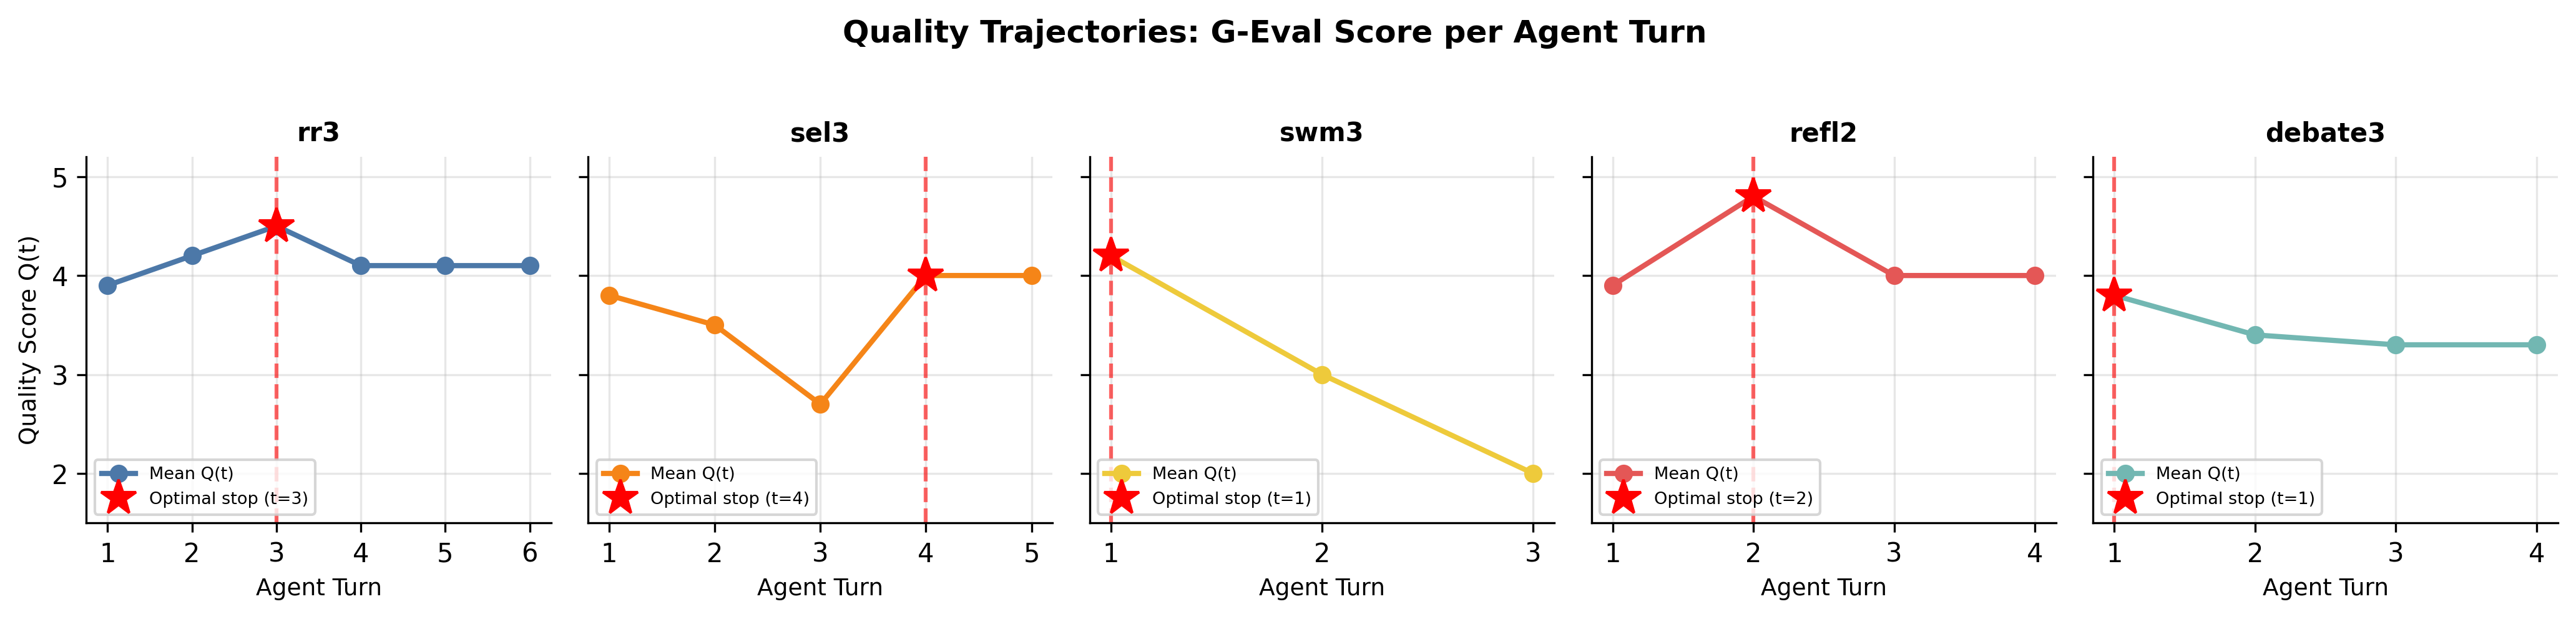
\includegraphics[width=\linewidth]{fig5_quality_trajectories.png}
\caption{Quality trajectories by topology. Refl2 peaks sharply at turn~2; debate3 declines monotonically; rr3 plateaus after turn~3.}
\label{fig:quality}
\end{figure}

\begin{figure}[H]
\centering
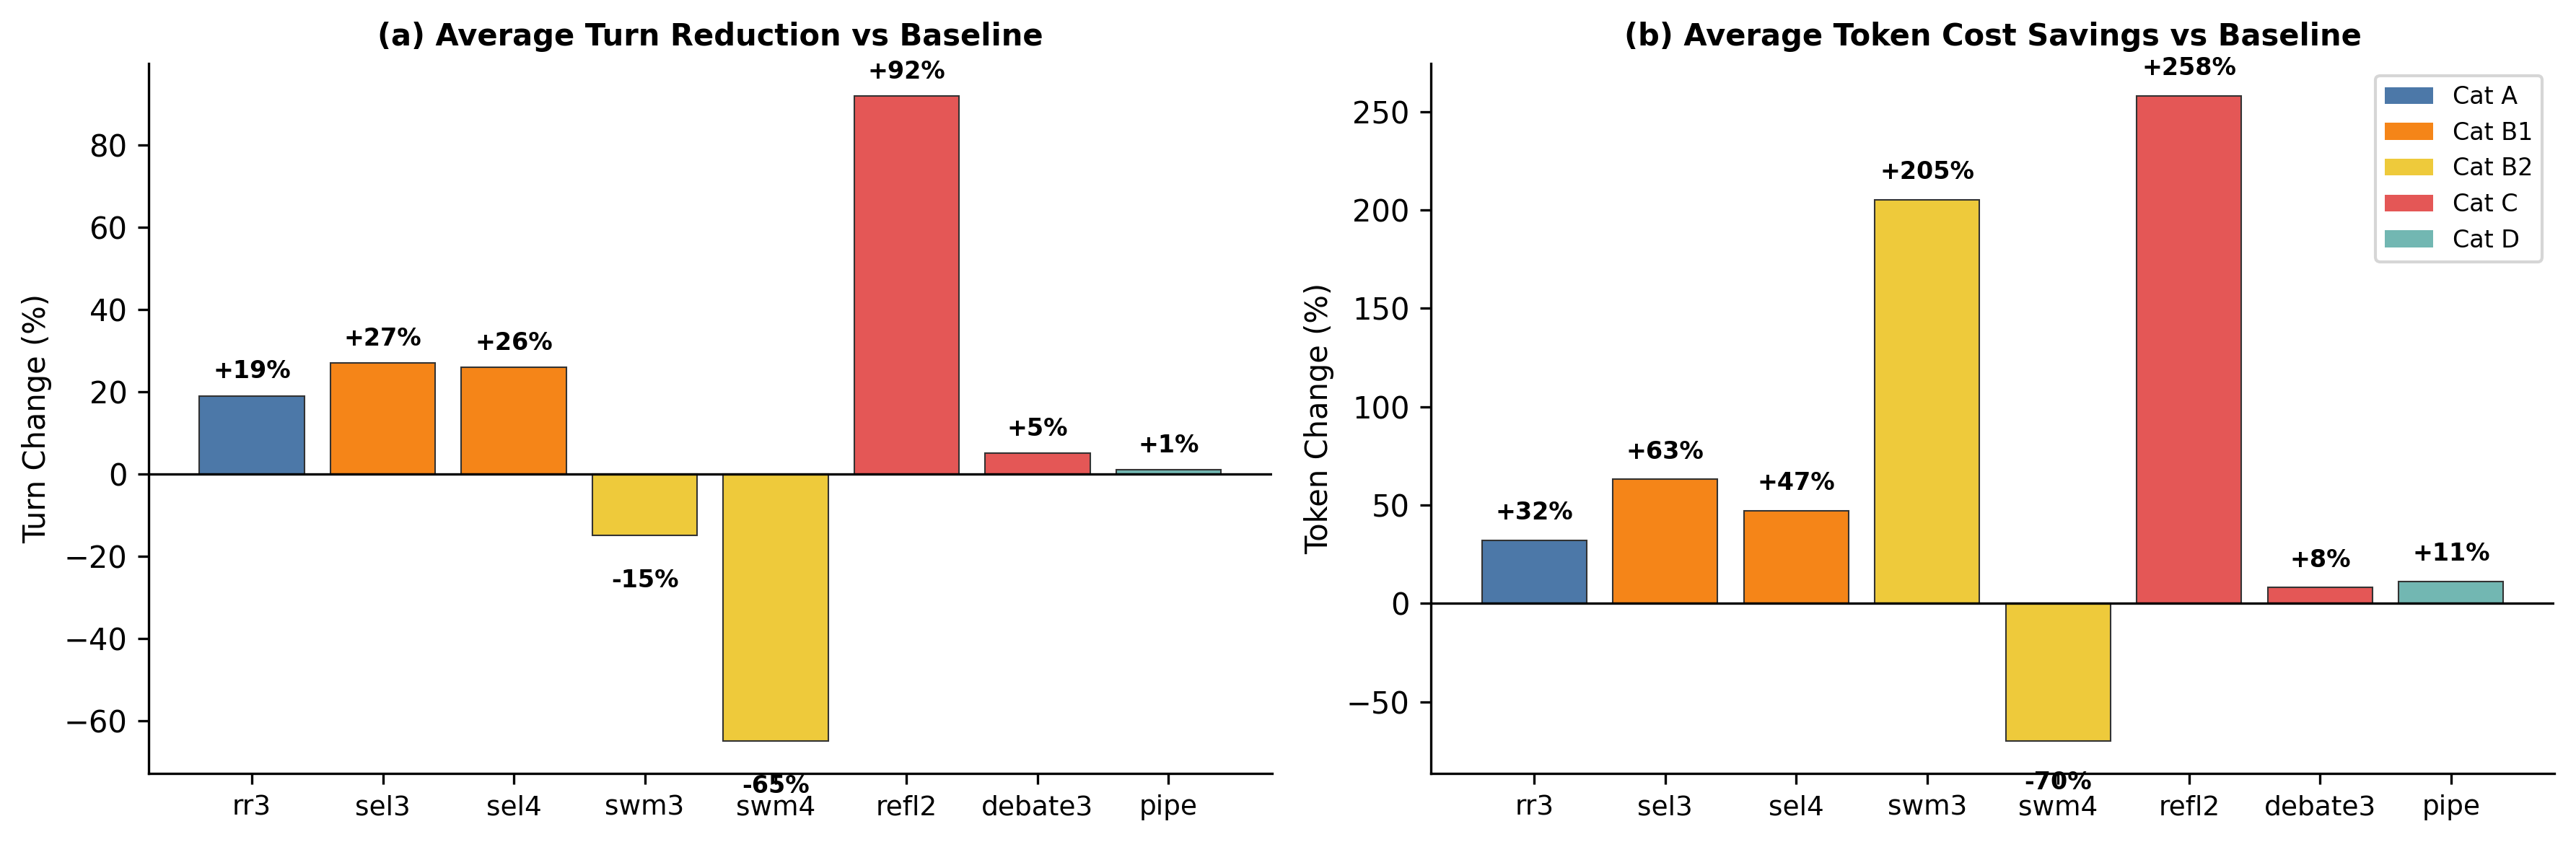
\includegraphics[width=\linewidth]{fig_exp05_savings_by_pattern.png}
\caption{Token savings from adaptive $\Delta U$ termination by pattern. swm4 shows dramatic savings; well-behaved patterns show minimal change.}
\label{fig:exp05}
\end{figure}

\begin{figure}[H]
\centering
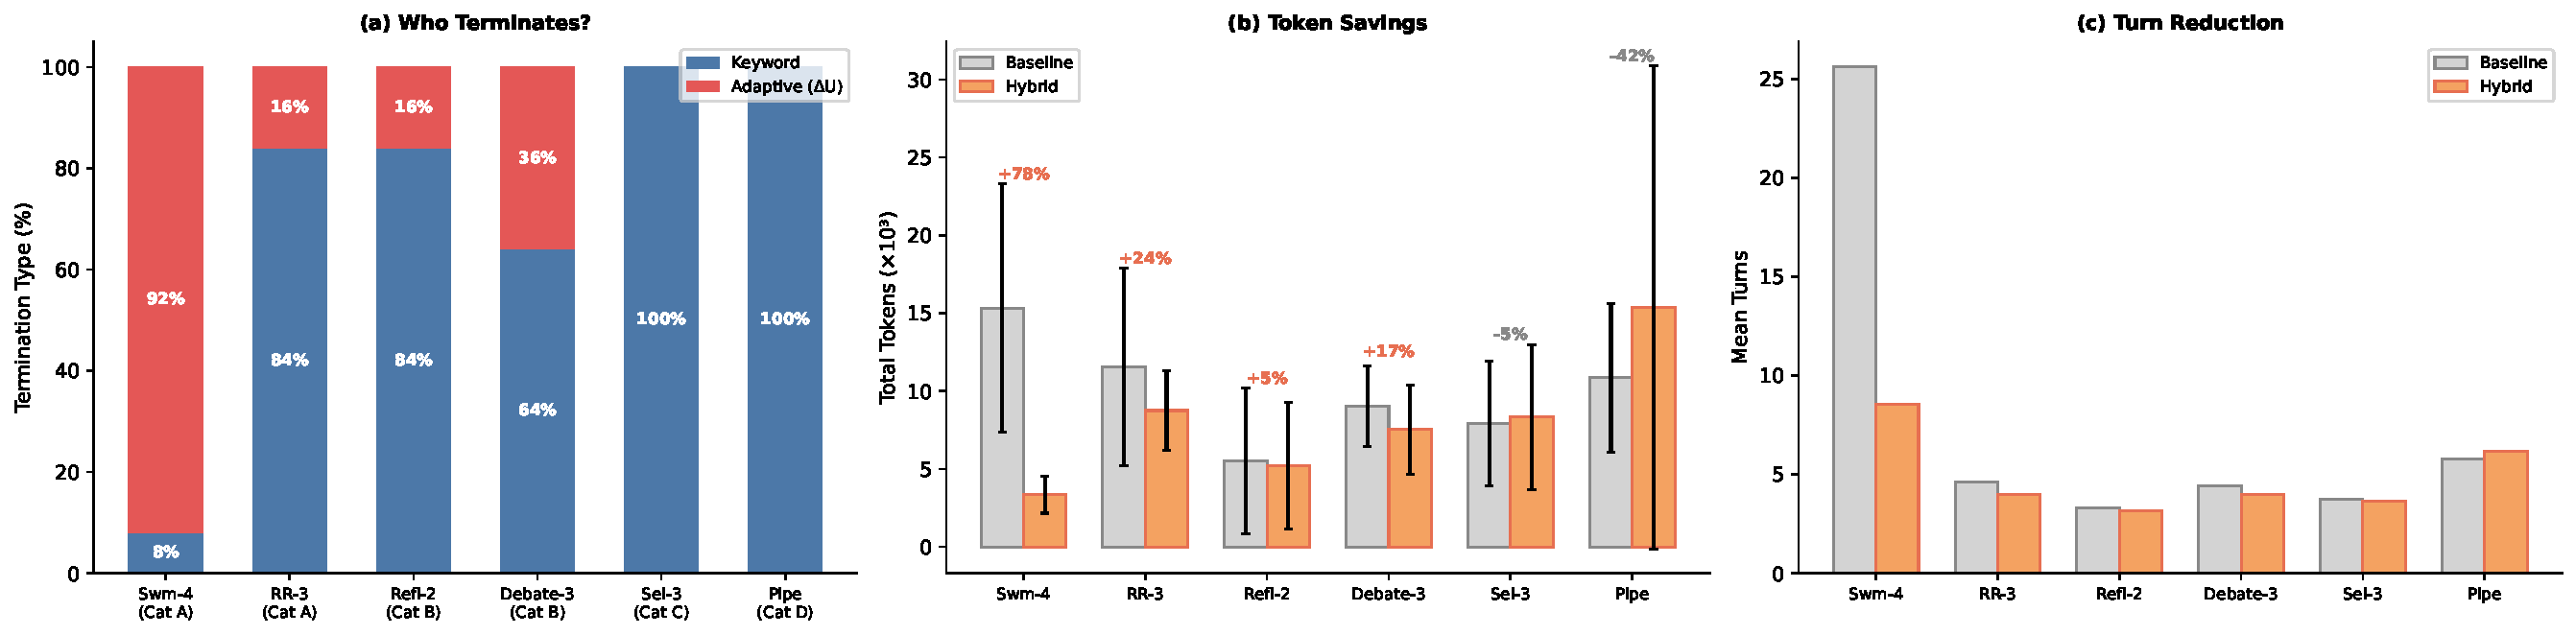
\includegraphics[width=\linewidth,height=6cm,keepaspectratio]{fig_hybrid_validation.pdf}
\caption{Hybrid termination validation across six patterns (categories A--D, 150 runs). (a)~$\Delta U$ dominates in swm4 (92\%); keyword dominates in sel3/pipe (100\%) and rr3/refl2 (84\%); debate3 mixed (64\% keyword). (b)~Token savings: swm4 78\%, rr3 24\%, debate3 17\%, refl2 5\%; keyword-only patterns show monitoring overhead (sel3 $-$5\%, pipe $-$42\%). (c)~Turn reduction mirrors token savings.}
\label{fig:hybrid}
\end{figure}

\section{Compressed Findings Summary}
\label{app:findings}

The 19 individual findings in the main text are organized into 17 core findings below. Original finding numbers are preserved in parentheses for cross-reference.

\begin{table*}[t]
\centering
\caption{Compressed findings: 19 individual observations $\to$ 17 core findings.}
\label{tab:compressed_findings}
\resizebox{\textwidth}{!}{
\begin{tabular}{@{}clll@{}}
\toprule
\textbf{\#} & \textbf{Core Finding} & \textbf{Orig.} & \textbf{Sec.} \\
\midrule
C1 & Multi-agent coordination incurs 3.3--17.4$\times$ token overhead; cost scales near-linearly; errors superlinearly & F1--2 & \ref{sec:exp01} \\
C2 & Centralized (B1) vs.\ decentralized (B2) routing produce radically different scaling: sub-linear vs.\ super-linear & F1--2 & \ref{sec:exp01} \\
C3 & swm3 (3 agents) achieves best token efficiency, beating even rr2 (2 agents): routing strategy $>$ agent count & F2 & \ref{sec:exp01} \\
C4 & Reflection \& debate exhibit opposite scaling; at equal count, reflection faster but debate cheaper per token & -- & \ref{sec:exp01} \\
C5 & Composed patterns (MoA, pipe) most expensive but highest output density per agent turn & -- & \ref{sec:exp01} \\
C6 & New cost hierarchy: $A \approx B2 < B1 \approx C \ll D$, replacing $A \ll B \approx C \ll D$ & -- & \ref{sec:exp01} \\
C7 & debate3 uniquely domain-invariant; task complexity amplifies cost 2$\times$ independently of topology & -- & \ref{sec:exp01} \\
C8 & Three quality trajectory shapes: monotone-plateau (rr3), peak-at-turn-2 (refl2), monotone-decline (debate3) & F3 & \ref{sec:exp02} \\
C9 & Termination regret varies 13$\times$ across topologies; reflection achieves near-zero quality loss & F4--5 & \ref{sec:exp02} \\
C10 & Semantic convergence (Sentence-BERT) reveals different ranking than surface metrics; feedback never converges & F6--7 & \ref{sec:exp03} \\
C11 & Three termination failure modes; factual tasks error-immune, technical error-prone; swarm structurally distinct & F8 & \ref{sec:exp04} \\
C12 & $\Delta U$ converges within 1.1--2.4 turns for all topologies; $\lambda$-insensitive (quality saturation dominates) & F9--11 & \ref{sec:exp05} \\
C13 & Adaptive termination benefit is topology-dependent: overhead for 7/8 patterns, $-$70\% for swm4 & F9--11 & \ref{sec:exp05} \\
C14 & Hybrid keyword+$\Delta U$ validated: preserves keyword efficiency, catches unreliable topologies & -- & \ref{sec:exp05} \\
C15 & Topology-dependent dynamics are model-invariant ($\rho$=0.762, $p$=0.028, $n$=8); routing efficiency model-sensitive & -- & \ref{sec:cross_model} \\
C16 & Topology features predict 54\% of token variance ($R^2$=0.54); $\texttt{agents} \times \texttt{max\_msg}$ is top predictor & F15--16 & \ref{sec:exp06} \\
C17 & Difficulty dominates pattern ($\eta^2_H$=0.364 vs.\ 0.046); solo dominance across 5/6 models on easy tasks; capability-dependent medium/hard benefits & F17--19 & \ref{sec:exp07} \\
\bottomrule
\end{tabular}
}
\end{table*}

\section{Difficulty-Graded Task Suite}
\label{app:difficulty_tasks}

\begin{table*}[t]
\centering
\caption{Difficulty-graded task suite (15 tasks for Experiment~07). Difficulty: easy=factual recall, medium=comparative analysis, hard=creative design with multi-constraint reasoning.}
\label{tab:difficulty_tasks}
\resizebox{\textwidth}{!}{
\begin{tabular}{@{}llllp{10cm}@{}}
\toprule
\textbf{ID} & \textbf{Domain} & \textbf{Diff.} & \textbf{Type} & \textbf{Task Description} \\
\midrule
sci\_easy & Science & Easy & Factual & Explain the first law of thermodynamics; what does conservation of energy mean in practice? \\
sci\_med & Science & Med & Analytical & Compare the three laws of thermodynamics with engineering applications for each \\
sci\_hard & Science & Hard & Creative & Design a novel waste heat recovery cycle beyond Rankine/Brayton with 1st/2nd law analysis \\
cs\_easy & CS & Easy & Factual & Explain client-server architecture: main components and communication \\
cs\_med & CS & Med & Analytical & Compare microservices vs.\ monolithic architecture across scalability, deployment, data consistency \\
cs\_hard & CS & Hard & Creative & Design migration strategy for 100K-DAU monolith to microservices with zero-downtime phasing \\
hist\_easy & History & Easy & Factual & List and explain three major causes of the fall of the Roman Empire \\
hist\_med & History & Med & Analytical & Compare decline of Roman Empire with British Empire (structural, economic, military factors) \\
hist\_hard & History & Hard & Creative & Develop general theory of imperial decline with falsifiable predictions for current global order \\
eng\_easy & Engineering & Easy & Factual & Explain dead loads vs.\ live loads in bridge engineering with examples \\
eng\_med & Engineering & Med & Analytical & Compare suspension vs.\ cable-stayed bridges for 500m+ spans \\
eng\_hard & Engineering & Hard & Creative & Design seismic-resistant bridge for tsunami-prone region (600m span, multi-hazard) \\
biz\_easy & Business & Easy & Factual & Explain venture capital: GP/LP roles, funding stages (seed through Series B) \\
biz\_med & Business & Med & Analytical & Compare VC funding vs.\ bootstrapping for B2B SaaS (growth, dilution, culture) \\
biz\_hard & Business & Hard & Creative & Design multi-stage funding strategy for deep-tech AI startup across 3+ ASEAN countries \\
\bottomrule
\end{tabular}
}
\end{table*}

\section{Six-Model Difficulty Replication}
\label{app:difficulty_6model}

\begin{table*}[t]
\centering
\caption{Six-model difficulty $\times$ pattern quality (mean G-Eval overall $\pm$ SD). Bold = highest per row. Models ordered by approximate capability (weak $\to$ strong). Haiku/GPT-4o-mini: 3 repeats per cell; others: 1 repeat.}
\label{tab:difficulty_6model}
\resizebox{\textwidth}{!}{
\begin{tabular}{@{}llccccc@{}}
\toprule
\textbf{Model} & \textbf{Diff.} & \textbf{Solo} & \textbf{Swm-3} & \textbf{Sel-3} & \textbf{Refl-2} & \textbf{Deb-3} \\
\midrule
Grok 3 Mini & Easy & \textbf{4.80}$\pm$.45 & 4.20$\pm$.45 & 3.40$\pm$.55 & 4.00$\pm$.71 & 2.40$\pm$.55 \\
 & Med & \textbf{3.00} & 2.80$\pm$.45 & 2.60$\pm$.55 & 2.80$\pm$.45 & 1.40$\pm$.55 \\
 & Hard & \textbf{2.60}$\pm$.55 & \textbf{2.60}$\pm$.55 & 2.40$\pm$.89 & 2.40$\pm$.55 & 1.60$\pm$.55 \\
\midrule
GPT-4o-mini & Easy & \textbf{4.79}$\pm$.43 & 4.73$\pm$.46 & 4.20$\pm$.77 & 4.20$\pm$.56 & 4.20$\pm$.68 \\
 & Med & \textbf{3.67}$\pm$.62 & 3.13$\pm$.64 & 3.13$\pm$.35 & 3.27$\pm$.46 & 3.00 \\
 & Hard & \textbf{3.00}$\pm$.53 & 2.93$\pm$.46 & 2.93$\pm$.26 & 2.93$\pm$.26 & 2.87$\pm$.35 \\
\midrule
Haiku 4.5 & Easy & \textbf{4.73}$\pm$.70 & 3.82$\pm$1.25 & 4.07$\pm$.88 & 4.67$\pm$.49 & 4.40$\pm$.63 \\
 & Med & 3.27$\pm$.46 & 3.80$\pm$1.01 & 3.33$\pm$.49 & \textbf{3.93}$\pm$.59 & 3.67$\pm$.72 \\
 & Hard & \textbf{3.67}$\pm$.98 & 3.00$\pm$.88 & 3.47$\pm$.74 & 3.47$\pm$.52 & 2.93$\pm$.46 \\
\midrule
Gemini 2.0 Flash & Easy & \textbf{4.80}$\pm$.45 & 4.00$\pm$1.73 & 3.40$\pm$.89 & 4.60$\pm$.55 & 3.00$\pm$.71 \\
 & Med & 3.40$\pm$.55 & 3.40$\pm$.55 & 3.40$\pm$.89 & \textbf{3.60}$\pm$.55 & 2.80$\pm$.45 \\
 & Hard & 3.00 & 3.00$\pm$.71 & 3.00 & \textbf{3.40}$\pm$.55 & 3.00 \\
\midrule
GPT-5.4 & Easy & \textbf{5.00} & 4.80$\pm$.45 & 4.80$\pm$.45 & \textbf{5.00} & 4.40$\pm$.89 \\
 & Med & 3.60$\pm$.55 & 3.40$\pm$.55 & 3.40$\pm$.55 & \textbf{4.60}$\pm$.55 & 3.20$\pm$.45 \\
 & Hard & 3.00 & 3.00 & 3.20$\pm$.45 & \textbf{3.80}$\pm$.84 & 3.00 \\
\midrule
Opus 4.6 & Easy & \textbf{5.00} & 4.25$\pm$.50 & 4.60$\pm$.55 & 4.60$\pm$.55 & 3.80$\pm$.45 \\
 & Med & 4.20$\pm$.45 & 3.80$\pm$.84 & 3.60$\pm$.55 & \textbf{4.40}$\pm$.89 & 3.00$\pm$.71 \\
 & Hard & 3.00 & 3.20$\pm$.45 & 3.00$\pm$.71 & \textbf{3.60}$\pm$1.14 & 2.60$\pm$.55 \\
\bottomrule
\end{tabular}
}
\end{table*}


\end{document}
